%!TEX root = ../../thesis.tex
\section{Generalized models for soft manipulators}
\label{sec: chap2 section header}
As mentioned previously, soft robots are composed of elastic bodies that can be  modeled as a dynamically deformable continuum with of infinite-dimensional nature. In this section, we aim to derive a compact and computationally efficient model that envelops the continuous dynamics of  the soft manipulator in Figure \ref{fig:C2:soft_robot} (and soft robotic systems of similar topology, \eg, \cite{Katzschmann2018,Falkenhahn2015,BibEntryOrm2019Sep}) through a  small set of generalized coordinates. We denote these coordinates by $\q\in\Q$. Their respective velocities are denoted by $\dq\in T_{\q}\Q$ which belong to the tangent space of the configuration manifold $\Q \subseteq \R^n$.  Let it be clear that the choice on $\q$ is free. However, finding a choice that minimizes $n = \dim(\q)$ and that accurately reflects the continuum nature can be challenging. A state representation that satisfies both will help to keep computational cost low which is the current bottleneck for model-based control of soft robots. 

We base our modeling framework on the work of Mochiyama et al. (2003, \cite{Mochiyama2003}), who outlined a theoretical foundation for continuum manipulators. Their work is extended upon by including extensibility, serial-chaining of multiple soft links, pneumatic actuation, and the introduction of nonlinear and time-dependent material behavior. Earlier modeling strategies addressing similar issues can be found in from Godage et al. (2016, \cite{Godage2015,Godage2016}), Della Santina et al. (2020, \cite{DellaSantina2020,DellaSantina2020a,DellaSantina2021}), Renda et al.
(2018, \cite{Renda2018}), and Boyer et al. (2021, \cite{Boyer2021}). Leveraging from the aforementioned works, a  finite-dimensional approximation of the true soft robot dynamics with  can be written in the familiar Lagrangian form:
%
\begin{align}
\MB(\q) \ddq + \vec{h}(\q,\dq) & = \vec{J}^\top\!(\q) \vec{\lambda} + \vec{\tau}(\q,\vec{u}), \label{eq:C2:model0}\\
\vec{\tau} & = \vec{G}^\top\!(\q) \vec{u},
\label{eq:C2:input_model0}
\end{align}
%
where $\MB(\q) \in \R^\nn$ denotes the generalized inertia matrix, $\vec{h}(\q,\dq) \in \R^n$ a vector of nonlinear state-dependent force contributions. The nonlinear state-dependent contributions possess a structures as follows: $\vec{h}(\q,\dq) = \vec{C}(\q,\dq)\dq + \vec{f}(\q,\dq)$  given by the Coriolis forces and visco-elastic terms, respectively.

\begin{asm}[Finiteness generalized inertia]
The generalized inertia matrix is a positive definite symmetric matrix that is bounded from both sides $\lambda^{-} \preceq \mat{M}(\q) \preceq \lambda^{+}$ for all configurations $\q$, where $\lambda^{-},\lambda^{+}$ are positive scalars.
\end{asm}

\begin{asm}[Passivity]
For any velocity $\dot{\q}$, it holds that $\dot{\q}^\top\left(\dot{\mat{M}} - 2\mat{C}  \right)\dot{\q} = 0$ -- the so-called passivity condition for Lagrangian systems. If the condition holds, it can easily be shown that map $\uB \mapsto \dot{\q}$ is passive, which implies that there exist a constant $\beta \ge 0$, such that the energy produced by the system $E^{\textrm{u}}$ is bounded from below \cite{Ortega1998}:
%
\begin{equation}
E^{\textrm{u}} := \int_0^T \dq^\top(\tau) \uB(\tau) \;d\tau > -\beta \quad \forall\,T > 0.
\label{as:C2:passivity}
\end{equation}
%
\end{asm}

\begin{asm}[Under-actuation]
In many cases, a soft robot that falls under the category hyper-redundant is also intrinsically under-actuated. Mathematically, under-actuation is defined as follows \cite{Russ2022}. A second-order system $\ddot{\q} = \fB(\q,\dq,\uB,t)$ is fully-actuated if, for any time $t$ and state $(\q,\dq)$, the flow map $\fB$ is surjective. In laymen's terms, for any acceleration $\ddot{\q}$ there is exists a unique input $\vec{u}$ that produces such response. Otherwise, the system is under-actuated. Given the control affine structure in \eqref{eq:C2:input_model0}, the system is under-actuated if configurations $\q \in \Q$ exist such that $\rank \left( \vec{G}(\q) \right) < \dim(\q)$. Let it be clear that fully-actuated systems are dramatically easier to control than under-actuated systems. However, for the sake of simplicity at this stage, we assume the actuation matrix to be full rank and time-invariant, \ie, $\vec{G}(\q) \simeq \vec{G}$. Under-actuation will be treated further in Chapter 4 and  is not considered here in Chapter 3 .
\end{asm}

In this chapter, a similar modeling framework is adopted to \cite{Mochiyama2003}; however, we propose an extension to incorporate FEM-driven data to more accurately reflect the underlying continuum mechanics -- in particular, hyper-elasticity and visco-elastic creep. We also propose a numerical scheme that significantly accelerates the computation of the continuous dynamics.
%
\begin{figure}[!t]
  \vspace{-5mm}
  \centering
  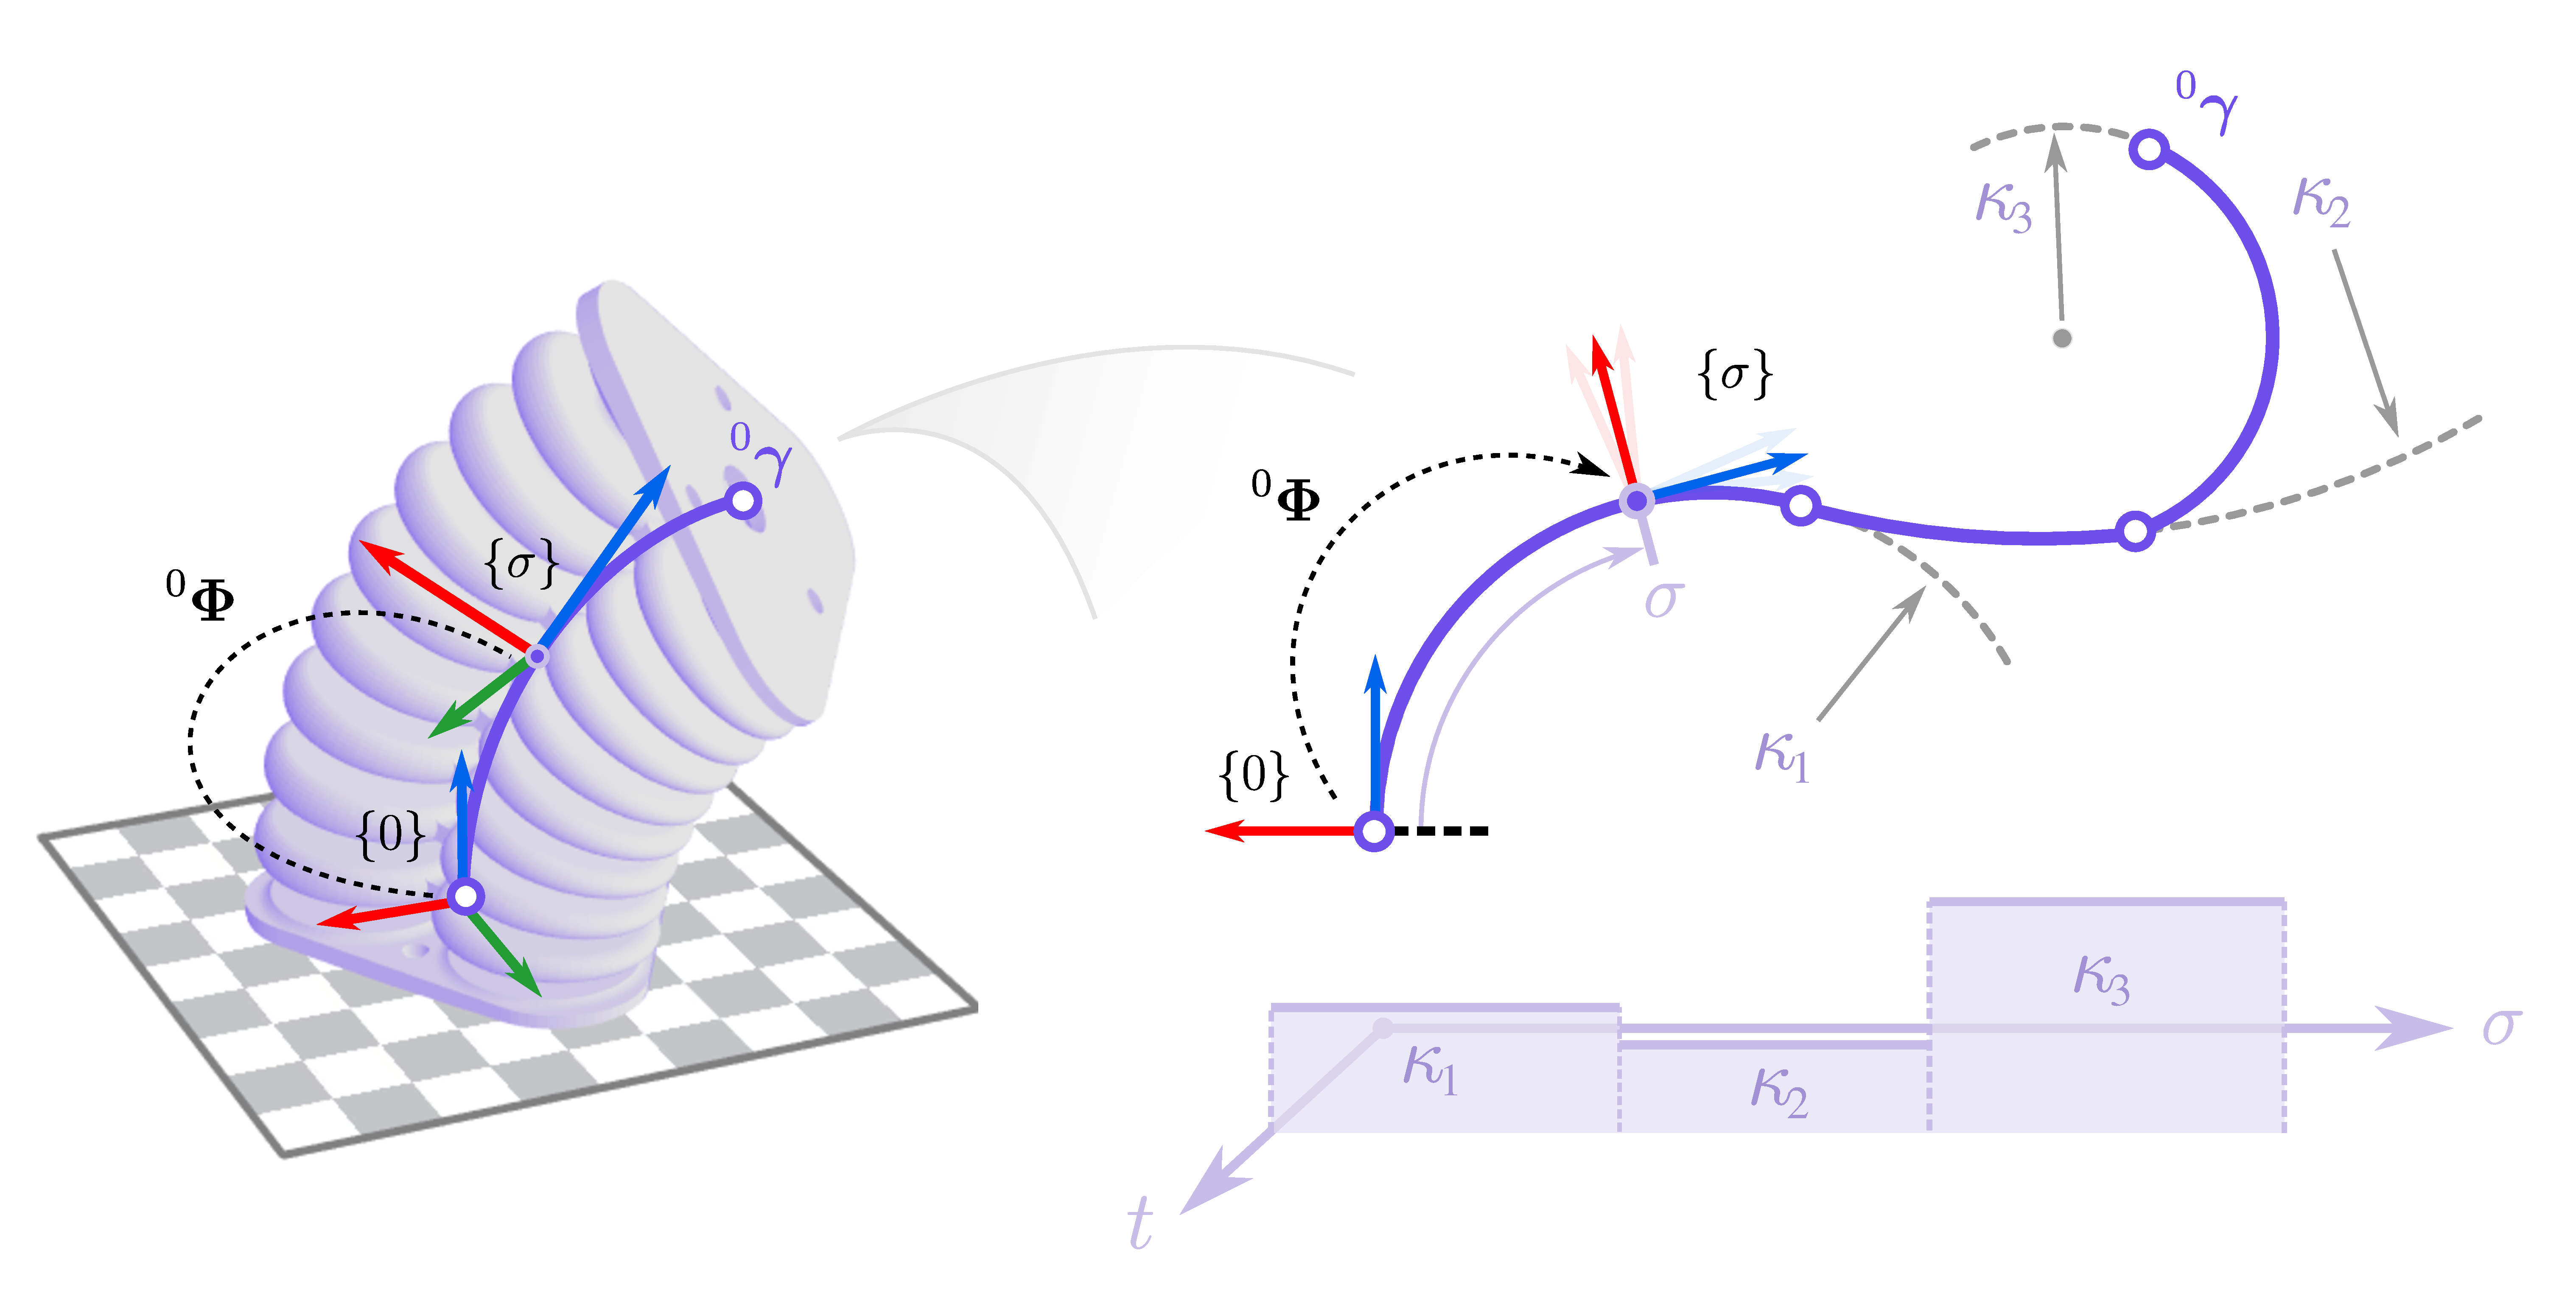
\includegraphics[width = \textwidth]{./pdf/thesis-figure-4-2.pdf}
  \caption{Schematic representation of the Piece-wise Constant Curvature (PCC) description for general soft  manipulator systems, given by a parameterized curve $^0 \gammaB: \Xs \times \mathcal{Q} \to \R^3$ and orientation matrix $^0 \PhiB: \Xs \times \mathcal{Q} \to \SO{3}$. The frame $\{\sigma\}$ is an inertial coordinate frame that evolves over the backbone $^0 \gammaB$ such that variations in $\sigma$ give insight into its differential geometry.}
  \label{fig:C2:configuration}
\end{figure}
%
\subsection{Piecewise curve kinematics}
\noindent To represent the hyper-flexible configuration of the soft robot, consider a smooth spatial curve that passes through the geometric center of the continuously deformable body, as shown in Figure \ref{fig:C2:configuration}. {In literature, this curve is called} the \textit{backbone curve} as it simplifies the three-dimensional deformation imposed by distributed forces acting on the elastic body. The arc-length of the backbone corresponds to the extensible length of the soft robot denoted by the variable $l(t)$ which we assume bounded ${l}_{-}\le l \le {l}_{+}$, and let $L$ be a constant denoting the {total unstressed} length of the soft robot. Next, let us introduce a spatial variable $\sigma \in \Xs$ that belongs to the one-dimensional material domain of the backbone curve, \ie, $\Xs = [0,\, L]$. Let it be clear that the spatial variable $\sigma$ represents the arc-length of a material coordinate along with the unstressed material domain of the soft robot manipulator.

Given each material coordinate, we wish to find a suitable low-dimensional  coordinate representation $\q$ such that the position vector $^0\gammaB(\sigma,\q)$ anywhere on the continuous backbone can be written as a mapping from generalized coordinates and space into Euclidean space $\R^3$:
%
\begin{equation}
^0\gammaB: \Xs \times \Q \to \R^3;
\end{equation}
%
and similarly the rotation matrix $^0\mat{\Phi}(\sigma,\vec{q})$ by a mapping from the generalized coordinates and space into $\SO{3}$:
%
\begin{equation}
^0\PhiB: \Xs \times \Q \to \SO{3}, \label{eq:phi_map}
\end{equation}
%
where {$\SO{3}$ denotes the special orthogonal group for rotations about the origin of $\R^3$}. Under this notion, the position vectors $^0\gammaB(0,\q)$ and $^0\gammaB(L,\q)$ relate to the base and the end-effector of the soft  manipulator, respectively. {Note tat left-sided superscript are used to indicate the frame of reference.} The set of all points on the backbone $\vec{\mathcal{C}} = \left\{\,^0\gammaB(\sigma,\q) \in \R^3~|~\sigma \in \Xs \right\}$ draws a possible {spatial} configuration of the soft robot given {a time instance $t \in \mathbb{T}$ on a finite horizon $\mathbb{T} = [0,T]$}.  For sake of brevity, the remainder of the chapter will drop the superscripts that indicate the frame of reference, \ie, $^0\PhiB = \PhiB$ and $^0\gammaB = \gammaB$.
%
\begin{asm}[Piece-wise Constant Curvature]
\label{asm:C2:pcc}
Despite the inherent flexibility in soft robotics, it is sometimes sufficient to express the kinematics according to the \emph{Piecewise Constant Curvature} (PCC) condition.  This properties often originates from the "\textit{proper}" structural design of the soft robot, where parasitic motion is reduced by structural compliance . Mathematically, it implies that the curvature of the continuous body satisfies $\kappa(\sigma_1,\q) = \kappa(\sigma_2,\q)$ for spatial coordinates on a local region on the soft manipulator $\sigma_1,\sigma_2 \subseteq \Xs$. As a result, this condition allows us to describe the full forward kinematics with a significantly reduced set of generalized coordinates, mitigating kinematic complexity in the model. Numerous works employ PCC models \cite{Falkenhahn2015,Katzschmann2019,Tatlicioglu2007,Marchese2016,Godage2016,DellaSantina2020a}, and depending on the elasticity  and structural geometry of the soft robot, the PCC condition has been proven to be consistent for various soft robotic systems.
\end{asm}
%
{Following this Constant Curvature (CC) approach, we assign a coordinate frame that twists minimally along the backbone -- formally called the "\textit{Bishop frame}" (see \cite{Bishop1975}) -- parametrized by the following generalized coordinate vector:}
%
\begin{equation}
\vec{q} := \begin{pmatrix}
\,\varepsilon & \kappa_x & \kappa_y\,
\end{pmatrix}^\top \in \mathcal{Q},
\label{eq:C2:coordinate}
\end{equation}
%
\noindent where $\varepsilon_{-} \le \varepsilon \le \varepsilon_{+}$ is the elongation strain, and $\kappa_x,\,\kappa_y\in\mathbb{R}$ are the curvatures or angular strains in $x$-$z$ and $y$-$z$ plane, respectively; and $\mathcal{Q} \subset \R^3$ is an admissible space on which $\q$ evolves. We will also introduce the following geometric variables $\kappa = \inner{\kappa_x}{\kappa_y}$ and the curvature angle $\phi = \atantwo(\kappa_y,\kappa_x)$. It is worth mentioning that the joint description above is somewhat related to Renda. et al. \cite{Renda2018} who proposed a \emph{Piece-wise Constant Strain} (PCS) parametrization with the exception of including the twist along the tangent.

By exploring the differential geometry of the smooth backbone curve similar to Mochiyama et al. \cite{Mochiyama2003}, we can write the position vector $\gammaB(\sigma,\q)$ and the orientation matrix $\PhiB(\sigma,\q)$ for each material point $\sigma$ along the smooth backbone as a differential equation:
%
\begin{align}
\renewcommand*{\arraystretch}{2}{}
\frac{\partial \,\!\mat{\Phi}}{\partial \sigma}(\sigma,\q) & = \, \mat{\Phi}(\sigma,\vec{q}) \,\mat{\Gamma}^{\times} (\sigma,\q), \label{eq:C2:change_phi} \\[0.75em]
%
\frac{\partial \, \gammaB}{\partial \sigma}(\sigma,\q) & = \, \mat{\Phi}(\sigma,\vec{q}) \, \vec{U}(\sigma,\q), \label{eq:C2:change_p}
\end{align}
%
where  $\vec{\Gamma}^\times \in \sog{3}$  is a skew-symmetric matrix composed of the entries of the vector $\vec{\Gamma} \in \R^3$, and $\vec{U}\in \R^3$ a vector representing the tangent along the extensible backbone. The skew-symmetric operator $(\,\cdot\,)^\times$ denotes the isomorphism between the Lie algebra $\sog{3}$ and $\R^3$. The vectors $\vec{\Gamma}$ and $\vec{U}$ are vectors that define the differential geometry of the backbone
\cite{Mochiyama2003} which are unique entries that live in the tangent space of the rigid-body transformation group (\ie, $T_{\SE{3}}$). Given the Bishop parametrization shown in \eqref{eq:C2:coordinate} and assuming the Piecewise Constant-Strain (PCC) condition, these geometric entities yield
%
\begin{align}
\vec{\Gamma}^\times(\sigma,t) & \simeq \vec{\Gamma}^\times(\sigma,\q(t)) \!\!\!\quad \xRightarrow[]{\textrm{\;\;PCC\;\;}}\quad \vec{\Gamma}^\times = \begin{pmatrix} 0 & 0 & \kappa_y \\ 0 & 0 & \kappa_x \\ -\kappa_y & -\kappa_x & 0 \end{pmatrix}, \label{eq:C2:Gamma}\\[0.35em]
%
\vec{U}(\sigma,t) & \simeq \vec{U}(\sigma,\q(t)) \!\quad \xRightarrow[]{\textrm{\;\;PCC\;\;}} \quad \;\; \vec{U} = \;\begin{pmatrix} \;0\;\; \\  \;0\;\; \\ \;\varepsilon + 1\;\ \end{pmatrix}. \label{eq:C2:U}
\end{align}
%
%with $\vec{U}^\circ$ the unit-tangent pointing, and $\vec{\Gamma}^\circ$ the intrinsic curvature/torsion of the curve. For simplicity, lets assume $\vec{U}^\circ = (0,0,1)^\top$ and $\vec{\Gamma}^\circ = \vec{0}_3$.
Now, given an initial configuration of backbone's base, \ie, $\mat{\Phi}(0,\vec{q}) = \vec{\Phi}_0$ and $ \gammaB(0,\q) = \vec{0}_3$, we can now solve for the position and orientation for each material coordinate $\sigma$ along the backbone:
%
\begin{align}
\mat{\Phi}(\sigma,\vec{q}) & = \vec{\Phi}_0\exp_{\SO{3}}(\sigma \vec{\Gamma}^\times(\vec{q})), \label{eq:C2:phi_exact} \\[0.35em]
\gammaB(\sigma,\vec{q}) & = \int_0^\sigma\,^0\mat{\Phi}(s, \vec{q})\, \vec{U}(\vec{q}) \; ds,
\label{eq:C2:pos_exact}
\end{align}
%
where $\exp_{\SO{3}}: \sog{3} \to \SO{3}$ is the exponential map. Luckily, there exists a compact expression for the exponential mapping related to the orthogonal group of rotation matrices $\SO{3}$ called the "\emph{Rodriguez formulas}".  The rotation angle along the soft body can be computed by $\theta(\sigma,\q) := \int_0^\sigma \kappa(s,\q) \; ds = \kappa(\q) \sigma$. Notice that the rotation angle $\theta$ linearly depends on $\sigma$, which is a property that follows from Assumption \ref{asm:C2:pcc}. Then, given the expression for the angle of rotation,  we can compactly rewrite the rotation matrix \eqref{eq:C2:phi_exact} in terms of $\cos(\theta)$ and $\sin(\theta)$ using these formulas as follows \cite{Lynch2017}:
%
\begin{equation}
\PhiB(\theta) = \PhiB_0 \left( \mat{I}_3 + \left[ \frac{\sin(\theta)}{\theta} \right]  \GammaB^{\times} + \left[ \frac{1-\cos(\theta)}{\theta^2} \right]  \GammaB^{\times} \GammaB^{\times} \right).
\label{eq:C2:phi_rodr}
\end{equation}
%
Note that the closed-form solutions \eqref{eq:C2:phi_exact} and \eqref{eq:C2:pos_exact} represent the forward configuration kinematics of the backbone curve. To express the forward velocity kinematic, let
$\etaB(\sigma,\q,\dq) = \left( \vec{\omega}^\top, \vec{v}^\top \right)^\top \in \R^6 \cong \seg{3}$
 be the aggregate of the angular velocity and linear velocity components relative to an inertial frame at $\sigma$, where the space $\seg{3}$ denotes the Lie algebra of $\SE{3}$. The velocity twist is computed by the following integration procedure:
%
\begin{align}
 \etaB(\sigma,\q,\dq)& = \Ad_{\mat{g}(\sigma,\cdot)}\inv \int_0^\sigma \Ad_{\mat{g}(s,\cdot)}\, \JB^\star\! \dq\;ds, \notag \\ & 
 \,=:\, \JB(\q,\sigma) \dq, \label{eq:C2:vel_cont}
\end{align}
%
where $\Ad_g: \SE{3} \to \mathbb{R}^{6\times 6}$ denotes the adjoint transformation matrix regarding the rigid body transformation $\gB \in \SE{3}$ that maps local velocities (i.e., twist) to a frame located at $\sigma$, and $\JB^\star:\Q \to T_{\q}\Q$ the joint-axis matrix that relates the DOFs to the generalized coordinate description. Let it be clear that the joint-axis matrix is naturally constant for a soft segment modeled with the Constant-Strain (CS) assumption. We will later relax this assumption in Chapter 4. Nevertheless here, the joint-axis matrix for an extensible and bendable CS segment parametrized by the Bishop parameters is given by
%
\begin{align}
\renewcommand*{\arraystretch}{1}{}
\JB^\star := \begin{pmatrix}\dfrac{\p \GammaB}{\p \q}^\top & \dfrac{\p \UB}{\p \q}^\top \end{pmatrix}^\top  = \begin{pmatrix}
\,0 & 0 & 0 & 0 & 0 & 1 \, \\
\,0 & 1 & 0 & 0 & 0 & 0 \,  \\
\,-1 & 0 & 0 & 0 & 0 & 0 \,  \\
\end{pmatrix}^\top. \label{eq:C2:joint-axis-matrix}
\end{align}
%
Although we based the forward kinematics on Mochiyama et al. (2003, \cite{Mochiyama2003}), the derived expression for the velocity twist in \eqref{eq:C2:vel_cont} is analogous to the work of Renda et al. (2018, 2020; \cite{Renda2018,Renda2020}), and Boyer et al. (2010, 2021; \cite{Boyer2010,Boyer2021}). Please also note that
\eqref{eq:C2:vel_cont} gives rise to the geometric Jacobian $\JB(\sigma,\q)$ that defines the mapping from joint velocities to the velocity twist anywhere on the body.

Given the explicit expression for the velocity twist in \eqref{eq:C2:vel_cont}, we can derive the acceleration twist \cite{Boyer2021,Mochiyama2003,Renda2018} which is obtained through differentiation of \eqref{eq:C2:vel_cont}:
%
\begin{align}
\dot{\etaB}(\sigma,\q,\dq,\ddq) & = \JB \ddot{\q} + \Ad_{\gB(\cdot,\sigma)} \inv \int_0^\sigma \Ad_{\gB(s,\cdot)}
\ad_{\etaB(s,\cdot,\cdot)} \, \JB^\star\! \dq \;ds \notag \\
& :=  \JB(\sigma,\q)\ddot{\q} + \dmat{J}(\sigma,\q,\dot{\q}) \dot{\q},
\label{eq:C2:acceleration}
\end{align}
%
where $\ad_{\etaB}: \R^{6} \to \R^{6\times 6}$ denotes the adjoint transformation regarding the velocity twist $\vec{\etaB}^\wedge \in \seg{3}$. The reader is referred to Appendix \ref{app:C2:adjoint} for more detailed expressions on the adjoint transformations.
%
\begin{rmk}[Numerical instability near zero-curvature] For many of the PCC modeling frameworks \cite{Falkenhahn2015}, there are mentions of a singularity point or discontinuity of the kinematic formulations at zero-curvature $\kappa = 0$. It is often reported that trajectories that pass through the origin lead to unbounded linear velocities $\vec{v} := \floor{\etaB}_3$, which may result in critical problems in practice. Although it is believed the problem is simply a by-product of the PCC hypothesis, this is however a common misconception, and it stems from a numerical origin. To illustrate this, consider the inextensible planar case: $\varepsilon = \kappa_y = 0$ and $\kappa = \kappa_x$.  For simplicity, we assume $L = 1$. Hence, by solving the forward kinematics for the position vector $\gammaB(\sigma,\kappa)$, and approaching zero-curvature from the positive domain $\kappa^{+} \to 0$, we see that
%
\begin{align}
\lim_{\kappa \to \,0^{+}}\gammaB(\sigma,\kappa) & = \begin{pmatrix} \dfrac{1-\cos(\sigma \kappa)}{\kappa}\,, & 0\,, & \dfrac{\sin(\sigma \kappa)}{\kappa} \end{pmatrix}^\top = \begin{pmatrix} 0 & 0 & \sigma \end{pmatrix}^\top,
\end{align}
%
so its limit clearly exists. Since the position vector $\gammaB$ is continuously differentiable when approaching the origin from both sides $\kappa \to 0^+$ and $\kappa \to 0^{-}$, it follows that $\dot{\gammaB}$ must be bounded for all $\kappa \in \Q$. We can simply check this by investigating the behavior of the linear-velocity components of the geometric Jacobian near zero-curvature, which yield
%
\begin{align}
\!\!\!\!\!\!\lim_{\kappa \to \,0^+} \floor{\JB}_3(\sigma,\kappa) & = \begin{pmatrix} \dfrac{\sigma \kappa \sin(\sigma \kappa) + 1 - \cos(\sigma \kappa)}{\kappa^2}, & 0, & \dfrac{\sigma \kappa \cos(\sigma \kappa) - \sin(\sigma \kappa) }{\kappa^2} \end{pmatrix}^\top \notag \\[0.75em] & = \begin{pmatrix} \sigma^2 & 0 & 0 \end{pmatrix}^\top.
\end{align}
%
 Again, its limit exists. Since both limits exist, we define $\vec{\gamma}(\sigma,0):= \lim_{\kappa \to \,0} \vec{\gamma}(\sigma,\kappa)$ and $\vec{J}(\sigma,0):= \lim_{\kappa \to \,0} \vec{J}(\sigma,\kappa)$. Consequently, the magnitude of the linear velocity of the end-effector reads simply $\lVert \dot{\gammaB}(L,\dot{\kappa}) \rVert = L^2\dot{\kappa} = L \omega_1$ with $\omega_1$ the angular velocity at the tip. Moreover, it is bounded for all $\kappa \in \mathcal{Q}$. This naturally poses an ambiguity on the origin of the kinematic singularity so often reported literature. The problem is believed to be of numerical origin when considering the zero-division. To make matters worse, deriving analytical expressions for accelerations will contain similar expressions that are hard to stabilize numerically. To resolve this issue, we opt for a numerical approximation of the forward kinematics -- namely, we employ an explicit forward integration scheme (\ie, trapezoidal integration) to solve \eqref{eq:C2:change_phi} and \eqref{eq:C2:change_p}.
\end{rmk}

\begin{figure}[!b]
  %% This file was created by matlab2tikz.
%
%The latest updates can be retrieved from
%  http://www.mathworks.com/matlabcentral/fileexchange/22022-matlab2tikz-matlab2tikz
%where you can also make suggestions and rate matlab2tikz.
%
\definecolor{mycolor1}{rgb}{0.06275,0.35686,0.84706}%
\definecolor{mycolor2}{rgb}{0.86667,0.21176,0.10980}%
\definecolor{mycolor3}{rgb}{0.18039,0.52157,0.25098}%
%
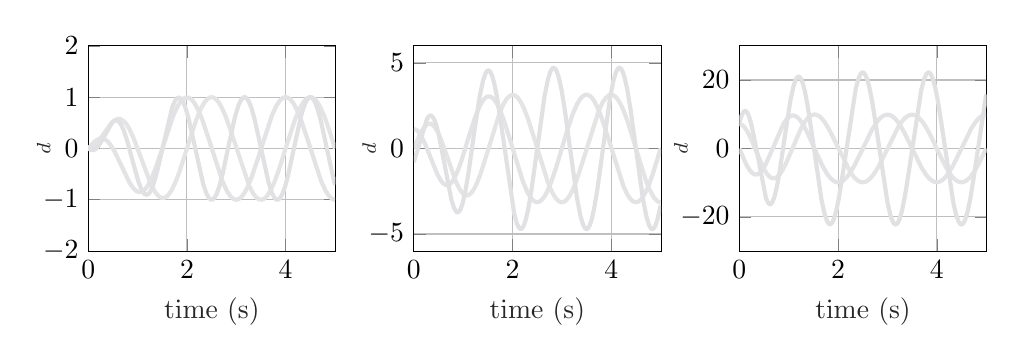
\begin{tikzpicture}

\begin{axis}[%
width=0.259\textwidth,
height=0.215\textwidth,
at={(0\textwidth,0\textwidth)},
scale only axis,
xmin=0,
xmax=5.01,
xlabel style={font=\color{white!15!black}},
xlabel={time (s)},
ymin=-2,
ymax=2,
ylabel style={font=\color{white!15!black}},
ylabel={$\q_d$},
axis background/.style={fill=white},
xmajorgrids,
ymajorgrids,
ylabel style={yshift=-9.5pt}
]
\addplot [color=mycolor1, line width=1.5pt, forget plot]
  table[row sep=crcr]{%
0	0\\
0.0590118023604722	0.0122599350151695\\
0.122024404880976	0.051245683586683\\
0.197039407881577	0.127356433673519\\
0.306061212242448	0.274610958461174\\
0.464092818563713	0.485281744378211\\
0.539107821564313	0.550009396707688\\
0.599119823964793	0.574155119595387\\
0.654130826165233	0.570918154822998\\
0.708141628325666	0.542425923995588\\
0.766153230646129	0.483585222567674\\
0.833166633326665	0.381001848782168\\
0.914182836567313	0.214127314579629\\
1.02820564112823	-0.075581754600881\\
1.25925185037007	-0.672851821290417\\
1.34526905381076	-0.833669846120815\\
1.41328265653131	-0.919160442883364\\
1.47129425885177	-0.95862945224353\\
1.52230446089218	-0.966293478371877\\
1.57331466293259	-0.948199994340202\\
1.62732546509302	-0.90137626204806\\
1.68933786757351	-0.814258548692571\\
1.76335267053411	-0.668276174824877\\
1.85537107421484	-0.435076623934572\\
1.99539907981596	-0.0143847160291388\\
2.19043808761752	0.562122882172909\\
2.28645729145829	0.78232701823107\\
2.36147229445889	0.906026029952742\\
2.4244848969794	0.971401468926922\\
2.47949589917984	0.997472999626086\\
2.53050610122024	0.995067322990411\\
2.58251650330066	0.966335526484759\\
2.63952790558112	0.905286120543856\\
2.70554110822164	0.798558894400302\\
2.78455691138228	0.62627694206536\\
2.8875775155031	0.345873241993202\\
3.26665333066613	-0.743113935603639\\
3.34566913382677	-0.884745361525436\\
3.41068213642729	-0.960888000773404\\
3.46669333866773	-0.994529710207253\\
3.51770354070814	-0.998453103672079\\
3.56871374274855	-0.976789847418135\\
3.624724944989	-0.924209595097784\\
3.68873774754951	-0.829302846512608\\
3.76375275055011	-0.675905403764888\\
3.85977195439088	-0.426427403766472\\
4.0128025605121	0.0402095863869585\\
4.1878375675135	0.556451691884553\\
4.28385677135427	0.778179781889043\\
4.35987197439488	0.904655728387877\\
4.42288457691538	0.970797027717512\\
4.47789557911582	0.997589797446857\\
4.52790558111622	0.996159624088327\\
4.57991598319664	0.968648768140962\\
4.6369273854771	0.908894839975858\\
4.70294058811762	0.803552513256307\\
4.78195639127826	0.632676263537522\\
4.88397679535907	0.356479989904654\\
5	8.88178419700125e-16\\
};
\addplot [color=mycolor2, line width=1.5pt, forget plot]
  table[row sep=crcr]{%
0	0\\
0.138027605521104	0.140440300108925\\
0.211042208441689	0.184935584810103\\
0.272054410882176	0.196656209080302\\
0.329065813162632	0.183310753811706\\
0.388077615523104	0.143577314476932\\
0.454090818163633	0.0688810755447316\\
0.533106621324265	-0.0570083146317186\\
0.645129025805161	-0.281096403013078\\
0.835167033406681	-0.662476511437434\\
0.916183236647329	-0.777169753245791\\
0.980196039207842	-0.832701926306017\\
1.03520704140828	-0.851571468783066\\
1.08621724344869	-0.843577250292476\\
1.13922784556911	-0.808789721087341\\
1.19823964792959	-0.739024227249642\\
1.26625325065013	-0.620955121877476\\
1.3502700540108	-0.427767812642783\\
1.46629325865173	-0.101666846450176\\
1.72234446889378	0.633525295214997\\
1.81136227245449	0.820837424693816\\
1.88337667533507	0.92640916650209\\
1.94338867773555	0.978331555991308\\
1.99639927985597	0.99518363496166\\
2.04740948189638	0.985184790347176\\
2.1004200840168	0.947820917223337\\
2.15943188637728	0.875183689696618\\
2.22844568913783	0.752107632272527\\
2.31346269253851	0.552461842844861\\
2.42848569713943	0.222651201302659\\
2.71854370874175	-0.633815634394776\\
2.80756151230246	-0.822691363947944\\
2.87857571514303	-0.928076540294048\\
2.93858771754351	-0.981414393680224\\
2.99159831966393	-0.999628398951698\\
3.04260852170434	-0.991037597553407\\
3.09561912382476	-0.955207840530338\\
3.15463092618524	-0.884300387785018\\
3.22364472894579	-0.7631603021345\\
3.30766153230646	-0.568142665295742\\
3.42068413682737	-0.246607234578534\\
3.72574514902981	0.65122625379941\\
3.8127625525105	0.831927524141501\\
3.88377675535107	0.93407870842546\\
3.94278855771154	0.983891068491499\\
3.99579915983197	0.999912900564358\\
4.04680936187237	0.989206735619766\\
4.0998199639928	0.951231137729379\\
4.15983196639328	0.876560868859253\\
4.22984596919384	0.750430990306204\\
4.31586317263453	0.546754312000056\\
4.43288657731546	0.209284340535875\\
4.71394278855771	-0.622647147364128\\
4.80396079215843	-0.816268101959198\\
4.87597519503901	-0.925047608943518\\
4.9369873974795	-0.980469837601955\\
4.98999799959992	-0.999506362945193\\
5	-0.999999999998463\\
};
\addplot [color=mycolor3, line width=1.5pt, forget plot]
  table[row sep=crcr]{%
0	-0\\
0.0590118023604722	-0.0323127302272486\\
0.108021604320864	-0.0331290824818566\\
0.157031406281257	-0.0079769875375062\\
0.212042408481697	0.0500216589361884\\
0.283056611322264	0.162185680095956\\
0.485097019403881	0.506055784611869\\
0.536107221444289	0.543684543712172\\
0.578115623124625	0.547118496091529\\
0.619123824764953	0.523782154432988\\
0.664132826565313	0.466781106891244\\
0.718143628725745	0.35651568991531\\
0.785157031406281	0.165020918099894\\
0.890178035607121	-0.209610885997843\\
1.02020404080816	-0.656165846278042\\
1.08621724344869	-0.813331876653166\\
1.13622724544909	-0.8827564770361\\
1.17623524704941	-0.902858557904033\\
1.21324264852971	-0.891876333186355\\
1.25225045009002	-0.849343403567872\\
1.29825965193039	-0.75980970794915\\
1.35527105421084	-0.595513228979666\\
1.43128625725145	-0.304509569554719\\
1.70234046809362	0.802351589692006\\
1.75935187037407	0.927771606903312\\
1.80436087217443	0.980075766519771\\
1.84136827365473	0.990077945444886\\
1.87737547509502	0.970779584879269\\
1.91838367673535	0.914613712496442\\
1.96739347869574	0.80264348414426\\
2.02940588117624	0.600183129717624\\
2.11542308461692	0.238476117081353\\
2.33046609321864	-0.696803833599685\\
2.39647929585917	-0.882732768124136\\
2.44748949789958	-0.969018921052845\\
2.4874974994999	-0.997830617495056\\
2.52250450090018	-0.994023401063271\\
2.55951190238048	-0.960649427962859\\
2.60252050410082	-0.885345365627133\\
2.65653130626125	-0.73993292743766\\
2.72654530906181	-0.482199139020603\\
2.83856771354271	0.0246624641119846\\
2.97559511902381	0.621277881997434\\
3.04660932186437	0.844169225727331\\
3.1006201240248	0.951944439490648\\
3.14362872574515	0.994104036503082\\
3.17963592718544	0.998126097022847\\
3.21564312862573	0.973479302424193\\
3.25665133026605	0.911429266327099\\
3.30666133226645	0.79016811146077\\
3.37067413482697	0.572402197653537\\
3.4626925385077	0.174902851173357\\
3.65173034606921	-0.655626629756043\\
3.72074414882977	-0.862521673164816\\
3.77275455091018	-0.959529089678471\\
3.81476295259052	-0.996173299612285\\
3.85077015403081	-0.996625968608955\\
3.8877775555111	-0.96726798143933\\
3.93078615723145	-0.896391559355475\\
3.98279655931186	-0.76204628869428\\
4.0498099619924	-0.523261917173079\\
4.15183036607321	-0.0698574757930102\\
4.30986197239448	0.62473490045429\\
4.38087617523505	0.846533085581687\\
4.43488697739548	0.953293435683277\\
4.47789557911582	0.994579768326681\\
4.51390278055611	0.997854639446826\\
4.55091018203641	0.971359701253584\\
4.59291858371674	0.905657492920928\\
4.64392878575715	0.778672904138067\\
4.70994198839768	0.549251284827934\\
4.80596119223845	0.128630790373577\\
4.97999599919984	-0.637409462896398\\
5	-0.707106781185458\\
};
\end{axis}

\begin{axis}[%
width=0.259\textwidth,
height=0.215\textwidth,
at={(0.341\textwidth,0\textwidth)},
scale only axis,
xmin=0,
xmax=5.01,
xlabel style={font=\color{white!15!black}},
xlabel={time (s)},
ymin=-6,
ymax=6,
ylabel style={font=\color{white!15!black}},
ylabel={$\dq_d$},
axis background/.style={fill=white},
xmajorgrids,
ymajorgrids,
ylabel style={yshift=-9.5pt}
]
\addplot [color=mycolor1, line width=1.5pt, forget plot]
  table[row sep=crcr]{%
0	0.00354490068904045\\
0.137027405481096	0.903588308385592\\
0.206041208241649	1.22856452598255\\
0.257051410282056	1.38060740669893\\
0.296059211842368	1.43857878332504\\
0.326065213042608	1.44671619310838\\
0.356071214242848	1.42249130990263\\
0.39007801560312	1.3560092907744\\
0.432086417283457	1.21821465698646\\
0.485097019403881	0.962586034545687\\
0.553110622124425	0.520529889641796\\
0.651130226045209	-0.270803972466815\\
0.857171434286857	-1.96111846971092\\
0.93118623724745	-2.39268873749415\\
0.988197639527906	-2.61578401240715\\
1.03220644128826	-2.71435218975166\\
1.06621324264853	-2.74427973959115\\
1.09621924384877	-2.73665215168262\\
1.12822564512903	-2.69342117279692\\
1.16623324664933	-2.59588760182128\\
1.21324264852971	-2.40873834185884\\
1.27225445089018	-2.07805095116542\\
1.34626925385077	-1.53498416704634\\
1.44928985797159	-0.609800554006279\\
1.7373474694939	2.06478538831989\\
1.81936387277455	2.60307834026396\\
1.88337667533507	2.90062171255517\\
1.93538707741548	3.05371910764113\\
1.97639527905581	3.11545185690039\\
2.00840168033607	3.12679834073453\\
2.03940788157632	3.10692697008051\\
2.0744148829766	3.04832587668127\\
2.11742348469694	2.92503238525876\\
2.16943388677736	2.70379607461824\\
2.23344668933787	2.33206311088885\\
2.31346269253851	1.73595350618949\\
2.42348469693939	0.745755428207096\\
2.72054410882176	-2.00968788046552\\
2.80556111222244	-2.57586752681016\\
2.87157431486297	-2.89102311132145\\
2.9245849169834	-3.05482622701098\\
2.96659331866373	-3.12471640436199\\
2.999599919984	-3.14152189462515\\
3.03060612122425	-3.12655715277568\\
3.06461292258452	-3.0760658872595\\
3.10662132426485	-2.96535682645882\\
3.15663132626525	-2.76652815312306\\
3.21864372874575	-2.42602567294836\\
3.29565913182637	-1.8771253886638\\
3.39767953590718	-0.987885846273739\\
3.75075015003001	2.23014715782088\\
3.82876575315063	2.70040323156362\\
3.89077815563113	2.96011198400992\\
3.93978795759152	3.08647630578385\\
3.97879575915183	3.13494797811861\\
4.01080216043209	3.1396111777881\\
4.04280856171234	3.11255800697227\\
4.07981596319264	3.04211546348687\\
4.124824964993	2.90122307727425\\
4.17983596719344	2.65075511896351\\
4.24684936987398	2.23986170977253\\
4.33186637327465	1.57905334730502\\
4.45289057811562	0.458374253608507\\
4.69693938787758	-1.82607588925665\\
4.7869573914783	-2.46688451700194\\
4.85697139427886	-2.83188138573282\\
4.9129825965193	-3.02625903108539\\
4.95799159831966	-3.11491811053946\\
4.99299859971994	-3.14093609486879\\
5	-3.14158748587636\\
};
\addplot [color=mycolor2, line width=1.5pt, forget plot]
  table[row sep=crcr]{%
0	1.12837322264768\\
0.0290058011602321	1.11287690718957\\
0.0620124024804962	1.05918703548886\\
0.103020604120824	0.940995733860333\\
0.154030806161233	0.720852429683366\\
0.221044208841769	0.329040615346998\\
0.324064812962592	-0.415015201309904\\
0.479095819163833	-1.51762477223098\\
0.550110022004401	-1.88091677154614\\
0.603120624124825	-2.05657754379251\\
0.643128625725145	-2.12690523971632\\
0.674134826965394	-2.14233493262017\\
0.703140628125626	-2.12518565975495\\
0.736147229445889	-2.06847786435016\\
0.776155231046209	-1.94764697173144\\
0.826165233046609	-1.72032118445276\\
0.888177635527105	-1.33287793109094\\
0.970194038807762	-0.677703297361942\\
1.1122224444889	0.656669942201704\\
1.25425085017003	1.92027334813605\\
1.33826765353071	2.4957239295581\\
1.40328065613123	2.8110209600663\\
1.45429085817163	2.96740997845937\\
1.49429885977195	3.03077028972536\\
1.52630526105221	3.04316268415615\\
1.55631126225245	3.0238292307504\\
1.59131826365273	2.96385353194767\\
1.63332666533307	2.84010088177006\\
1.68533706741348	2.61261209274866\\
1.74934986997399	2.23016785497343\\
1.83036607321464	1.61058449856721\\
1.94538907781556	0.55355301879334\\
2.20544108821764	-1.88333064164048\\
2.29345869173835	-2.49961881538618\\
2.3624724944989	-2.85081712197516\\
2.41748349669934	-3.03514561937135\\
2.46149229845969	-3.11735537496245\\
2.49549909981996	-3.14000923889623\\
2.52650530106021	-3.12935139813733\\
2.56051210242048	-3.08346030159967\\
2.6005201040208	-2.9844099202232\\
2.6505301060212	-2.79450937790965\\
2.71154230846169	-2.47007506810393\\
2.78655731146229	-1.94858631705674\\
2.88457691538308	-1.10996961666554\\
3.10262052410482	0.99996718143458\\
3.22164432886577	2.01874975626282\\
3.30566113222645	2.57684537272085\\
3.37167433486697	2.89165495774407\\
3.4246849369874	3.05520852382526\\
3.46669333866773	3.12491681950401\\
3.499699939988	3.14158841415858\\
3.53070614122825	3.12650471358071\\
3.56471294258852	3.07589032073885\\
3.60672134426885	2.96503961364553\\
3.65673134626925	2.76605754535741\\
3.71874374874975	2.42538893386612\\
3.79575915183037	1.87632266950521\\
3.89777955591118	0.986940126259217\\
4.25085017003401	-2.23084317749245\\
4.32886577315463	-2.70090796640865\\
4.39087817563513	-2.96044270093426\\
4.43988797759552	-3.08666036495903\\
4.47889577915583	-3.13501205318945\\
4.51090218043609	-3.13957601885231\\
4.54290858171634	-3.11242397791472\\
4.57991598319664	-3.04186887567698\\
4.624924984997	-2.9008442325007\\
4.67993598719744	-2.65022515672919\\
4.74694938987798	-2.23916940295443\\
4.83196639327866	-1.57819986384533\\
4.95299059811962	-0.457397634949563\\
5	0.00493479812624376\\
};
\addplot [color=mycolor3, line width=1.5pt, forget plot]
  table[row sep=crcr]{%
0	-0.794115508462454\\
0.0580116023204642	-0.277364611734568\\
0.26505301060212	1.70491593082617\\
0.306061212242448	1.87842338112035\\
0.334066813362672	1.92300384411942\\
0.356071214242848	1.91292691038186\\
0.38007601520304	1.85542433262415\\
0.411082216443289	1.70919219099674\\
0.451090218043609	1.40465740373763\\
0.504100820164033	0.820935563376146\\
0.578115623124625	-0.248600075058891\\
0.762152430486097	-2.99671953899652\\
0.816163232646529	-3.4867860854134\\
0.855171034206841	-3.68308225183768\\
0.882176435287057	-3.73307210749446\\
0.902180436087217	-3.72294329754286\\
0.924184836967394	-3.66485742913014\\
0.954190838167634	-3.50676773602809\\
0.993198639727946	-3.16939676216821\\
1.04320864172835	-2.53683562435458\\
1.11022204440888	-1.40251215395337\\
1.23224644928986	1.09146932720294\\
1.34026805361072	3.11962860739989\\
1.40428085617123	3.97847580467464\\
1.45229045809162	4.38259317834563\\
1.4872974594919	4.53109137402165\\
1.51030206041208	4.55856842712607\\
1.53030606121224	4.53675451436047\\
1.55431086217243	4.45469330662973\\
1.58631726345269	4.25233666981845\\
1.62832566513303	3.83346415954477\\
1.68233646729346	3.06612040251519\\
1.75535107021404	1.70902193090805\\
2.03440688137628	-3.80704018778977\\
2.08841768353671	-4.38067909824091\\
2.12942588517704	-4.62780828971085\\
2.15843168633727	-4.6982027777484\\
2.17843568713743	-4.69538596539201\\
2.1994398879776	-4.64729630338051\\
2.22744548909782	-4.5121578146679\\
2.26445289057812	-4.21315733318806\\
2.3124624924985	-3.63571053810641\\
2.374474894979	-2.61980512471882\\
2.46549309861972	-0.754128407877475\\
2.6495299059812	3.05964290826855\\
2.71654330866173	4.02147655398821\\
2.76655331066213	4.48381747958504\\
2.80356071214243	4.66721925102645\\
2.82956591318264	4.71152470359658\\
2.84856971394279	4.69919553002523\\
2.87157431486297	4.63390058682298\\
2.90158031606321	4.46715113358115\\
2.94058811762353	4.11776373765277\\
2.99059811962393	3.4689862272862\\
3.05761152230446	2.30691776642933\\
3.16363272654531	0.0563190270418401\\
3.30666133226645	-2.89690138385146\\
3.37667533506701	-3.9448221542987\\
3.42868573714743	-4.45241981565303\\
3.46769353870774	-4.65954561876156\\
3.49469893978796	-4.71117486462973\\
3.51470294058812	-4.70029361858979\\
3.53670734146829	-4.64013279511158\\
3.56671334266853	-4.47797683817697\\
3.60572114422885	-4.13425107699655\\
3.65573114622925	-3.49192821143007\\
3.72174434886977	-2.35576737664234\\
3.82576515303061	-0.156931641015601\\
3.97379475895179	2.90509369151093\\
4.04380876175235	3.950496362776\\
4.09581916383277	4.45581244484655\\
4.13482696539308	4.66108744519533\\
4.16183236647329	4.71140168604915\\
4.18183636727345	4.69954306835578\\
4.20484096819364	4.63434132500523\\
4.23484696939388	4.46772453283112\\
4.27385477095419	4.11851887812703\\
4.32386477295459	3.46996990086312\\
4.39087817563513	2.30815865696121\\
4.49689937987598	0.0577494594312666\\
4.63992798559712	-2.89575760597693\\
4.70994198839768	-3.94402589682519\\
4.7619523904781	-4.45194298479568\\
4.80096019203841	-4.65932964437099\\
4.82796559311862	-4.71114488543943\\
4.84796959391878	-4.70040215831249\\
4.86997399479896	-4.64039276611033\\
4.8999799959992	-4.47843880303433\\
4.93898779755951	-4.13496168317129\\
4.98899779955991	-3.49292197179463\\
5	-3.32429866327344\\
};
\end{axis}

\begin{axis}[%
width=0.259\textwidth,
height=0.215\textwidth,
at={(0.682\textwidth,0\textwidth)},
scale only axis,
xmin=0,
xmax=5.01,
xlabel style={font=\color{white!15!black}},
xlabel={time (s)},
ymin=-30,
ymax=30,
ylabel style={font=\color{white!15!black}},
ylabel={$\ddq_d$},
axis background/.style={fill=white},
xmajorgrids,
ymajorgrids,
ylabel style={yshift=-9.5pt}
]
\addplot [color=mycolor1, line width=1.5pt, forget plot]
  table[row sep=crcr]{%
0	7.08971722508816\\
0.0170034006801352	7.06254176227866\\
0.0380076015203041	6.96211357748433\\
0.0670134026805353	6.70383363218785\\
0.105021004200839	6.16331809076554\\
0.15503100620124	5.13123086154366\\
0.221044208841768	3.30313004756611\\
0.322064412882577	-0.140715150531712\\
0.483096619323865	-5.57492932673487\\
0.555111022204441	-7.34242512612227\\
0.609121824364873	-8.2298345369658\\
0.650130026005201	-8.61942170460317\\
0.679135827165434	-8.74010611151554\\
0.696139227845569	-8.75056964311227\\
0.714142828565713	-8.71323899853671\\
0.738147629525905	-8.58686459570546\\
0.770154030806161	-8.28547401565682\\
0.812162432486497	-7.67074463808859\\
0.866173234646929	-6.54917377090891\\
0.937187437487498	-4.60734590265721\\
1.04320864172835	-1.07483524322571\\
1.24624924984997	5.72961331213317\\
1.32926585317063	7.81639650559995\\
1.39427885577116	8.9859331390274\\
1.44528905781156	9.58253887084481\\
1.48529705941188	9.8442837551671\\
1.51330266053211	9.91865276034343\\
1.53230646129226	9.91831589369774\\
1.55331066213243	9.87066630009359\\
1.58031606321264	9.73764473499728\\
1.61632326465293	9.43822354992907\\
1.6623324664933	8.86253703324957\\
1.72034406881376	7.8537245560284\\
1.79335867173435	6.19915830635254\\
1.89137827565513	3.47504190478798\\
2.25345069013803	-7.05759085861679\\
2.32946589317864	-8.49825043913732\\
2.39047809561912	-9.30375995789046\\
2.4374874974995	-9.69098733938356\\
2.47349469893979	-9.84429919326235\\
2.49849969993999	-9.87645177319418\\
2.51850370074015	-9.85815891485498\\
2.54250850170034	-9.78470810142351\\
2.5745149029806	-9.6001934501988\\
2.61552310462092	-9.22223443122761\\
2.66653330666133	-8.53959500779489\\
2.72954590918184	-7.39663922633138\\
2.80856171234247	-5.56189473532864\\
2.91558311662332	-2.55857583281172\\
3.22764552910582	6.49527125262672\\
3.30966193238648	8.17448519252473\\
3.374674934987	9.12633838257015\\
3.42568513702741	9.60899637547641\\
3.46469293858772	9.81236106656347\\
3.49269853970794	9.86769341093652\\
3.5127025405081	9.86048208595491\\
3.53570714142829	9.80407057871169\\
3.56471294258852	9.66005045055507\\
3.60272054410882	9.35027485493567\\
3.65073014602921	8.7694054033971\\
3.70974194838968	7.78440013127213\\
3.78275655131026	6.20094073200406\\
3.87877575515103	3.63970724426288\\
4.05881176235247	-1.84364405983484\\
4.19783956791358	-5.77205567675598\\
4.2868573714743	-7.75761622429094\\
4.35587117423485	-8.88854079805768\\
4.41088217643529	-9.49382693860024\\
4.45389077815563	-9.77065608576133\\
4.48489697939588	-9.85991079216486\\
4.50590118023605	-9.86727677343424\\
4.52690538107622	-9.83169388013572\\
4.55391078215643	-9.72310658142739\\
4.58891778355671	-9.47842189369386\\
4.63392678535707	-8.99611634308517\\
4.68893778755751	-8.16403545489397\\
4.75695139027806	-6.80236720584926\\
4.84396879375875	-4.61913345423115\\
4.97299459891978	-0.805433305647973\\
5	0.0310062018553658\\
};
\addplot [color=mycolor2, line width=1.5pt, forget plot]
  table[row sep=crcr]{%
0	-0.0356665298542058\\
0.14002800560112	-4.67099677947669\\
0.210042008401681	-6.35787080027761\\
0.262052410482097	-7.18121414389206\\
0.301060212042408	-7.52419844540775\\
0.328065613122625	-7.61679085886646\\
0.34506901380276	-7.61344158614619\\
0.364072814562913	-7.55338671970529\\
0.390078015603121	-7.3759254387018\\
0.425085017003401	-6.96795293714247\\
0.47009401880376	-6.17536023821841\\
0.528105621124224	-4.76203193936642\\
0.608121624324864	-2.2616035058598\\
0.90118023604721	7.41655342073599\\
0.965193038607721	8.68477119764233\\
1.01520304060812	9.31550428917571\\
1.05321064212843	9.57115136568376\\
1.07921584316863	9.63325353187106\\
1.09821964392879	9.62095442347266\\
1.12022404480896	9.54664003094408\\
1.14922984596919	9.35230091148043\\
1.1872374474895	8.93817915492701\\
1.23624724944989	8.15570308454472\\
1.29825965193039	6.81305056038362\\
1.38127625525105	4.53205984490834\\
1.51730346069214	0.137104630163254\\
1.6873374674935	-5.19413042832095\\
1.77835567113423	-7.44111083206267\\
1.8493698739748	-8.73764863851267\\
1.90638127625525	-9.44363453025954\\
1.95139027805561	-9.77614657982073\\
1.98439687937588	-9.89060722533797\\
2.00640128025605	-9.90571841918975\\
2.02640528105621	-9.87708129185361\\
2.05241048209642	-9.77998577411654\\
2.08541708341668	-9.56077689839852\\
2.12842568513703	-9.11882330623115\\
2.18143628725745	-8.34382797509914\\
2.24744948989798	-7.05721408722493\\
2.33146629325865	-4.99130619335819\\
2.45249049809962	-1.45521934033521\\
2.69453890778156	5.68634972386572\\
2.78455691138228	7.71289662082619\\
2.85457091418284	8.87123751025509\\
2.90958191638328	9.48327346161904\\
2.95259051810362	9.76549714637454\\
2.98459691938388	9.86011816772603\\
3.00560112022404	9.86808705516484\\
3.02660532106421	9.83309714619462\\
3.05361072214443	9.72525700271287\\
3.08861772354471	9.48151268853614\\
3.13262652530506	9.01304744316267\\
3.1876375275055	8.18694988291568\\
3.25565113022605	6.83174606330716\\
3.34266853370674	4.65484935746607\\
3.47069413882777	0.876546802294875\\
3.6877375475095	-5.51511477797639\\
3.77975595119024	-7.61957450245987\\
3.85077015403081	-8.81865742330401\\
3.90678135627125	-9.45828980758456\\
3.95079015803161	-9.75661509139414\\
3.98279655931186	-9.85681253462545\\
4.00480096019204	-9.86795820689945\\
4.02580516103221	-9.8346227153101\\
4.05281056211242	-9.72890484618461\\
4.0868173634727	-9.4963693895167\\
4.13082616523305	-9.03523157269603\\
4.18483696739348	-8.23480517953001\\
4.25185037007402	-6.91608604630467\\
4.33686737347469	-4.81255275530668\\
4.46089217843569	-1.17876018750085\\
4.69093818763753	5.59713704895159\\
4.78195639127826	7.66275629837665\\
4.85197039407882	8.8353040648137\\
4.90798159631926	9.46885282937515\\
4.95199039807962	9.76215955428295\\
4.98399679935987	9.85863512259488\\
5	9.86954757942193\\
};
\addplot [color=mycolor3, line width=1.5pt, forget plot]
  table[row sep=crcr]{%
0	7.5744225756329\\
0.0520104020804162	9.85795253565652\\
0.0890178035607114	10.7343646901029\\
0.113022604520904	10.9368263420187\\
0.126025205041007	10.9227666810555\\
0.142028405681135	10.7856109086146\\
0.16503300660132	10.3588706857098\\
0.197039407881576	9.32929431048124\\
0.240048009601921	7.21344321073802\\
0.300060012002401	3.12899615273476\\
0.541108221644329	-14.5767064028135\\
0.583116623324663	-15.8947102220086\\
0.611122224444888	-16.2686397032763\\
0.622124424884976	-16.3000792190449\\
0.634126825365072	-16.2590964666309\\
0.651130226045208	-16.0662320020655\\
0.67613522704541	-15.4974275623498\\
0.710142028405681	-14.1945663307275\\
0.75515103020604	-11.6027109979822\\
0.816163232646531	-6.78180501212378\\
0.918183636727345	3.19925678471389\\
1.0372074414883	14.2630289394763\\
1.1002200440088	18.3769434543013\\
1.14622924584917	20.2284519962292\\
1.17923584716943	20.8825917599187\\
1.19923984796959	20.9940018330856\\
1.21024204840968	20.9627983709382\\
1.22624524904981	20.8005305254444\\
1.25025005001	20.300173284471\\
1.28325665133027	19.1232943641539\\
1.32726545309062	16.7321518603769\\
1.38527705541108	12.3448435289664\\
1.46929385877175	4.24762456605077\\
1.66433286657331	-15.006835410114\\
1.72834566913383	-19.2314865141707\\
1.77635527105421	-21.2288700042196\\
1.81136227245449	-21.9820872663368\\
1.83336667333467	-22.1406342791886\\
1.84536907381476	-22.1238119583189\\
1.86137227445489	-21.9881962890689\\
1.88437687537508	-21.5687174401902\\
1.91638327665533	-20.5551161436279\\
1.95839167833567	-18.5063456770163\\
2.01340268053611	-14.7274455786217\\
2.08841768353671	-8.02930998083884\\
2.35847169433887	17.4889091607566\\
2.41448289657932	20.4580950794453\\
2.45649129825965	21.7593237376024\\
2.48549709941988	22.1621020797258\\
2.49949989997999	22.2084088691288\\
2.51150230046009	22.1710021117705\\
2.52850570114023	21.9964824567098\\
2.55351070214043	21.4835583106643\\
2.5875175035007	20.3092524488913\\
2.63252650530106	17.9608482179239\\
2.69053810762152	13.7652243370479\\
2.77155431086217	6.27861523427864\\
3.00360072014403	-16.0384936526148\\
3.06461292258452	-19.7357108331353\\
3.11062212442489	-21.463698030133\\
3.14362872574515	-22.0870363960568\\
3.16463292658532	-22.2064523468513\\
3.17663532706541	-22.1770731289039\\
3.19263852770554	-22.0276153410914\\
3.21664332866573	-21.5691020724051\\
3.249649929986	-20.4902631329995\\
3.29265853170634	-18.3476492789936\\
3.34866973394679	-14.44841849918\\
3.4256851370274	-7.52047923802124\\
3.68573714742949	17.1151521202173\\
3.74374874974995	20.2996418279255\\
3.78675735147029	21.6963760554245\\
3.81676335267053	22.146824126934\\
3.83276655331066	22.2065248116632\\
3.84476895379076	22.1684518725285\\
3.86177235447089	21.9932254539312\\
3.88677735547109	21.479711348027\\
3.92078415683137	20.3053143584819\\
3.96579315863173	17.9577095353878\\
4.02380476095219	13.7639924762123\\
4.10482096419284	6.28037173283591\\
4.3368673734747	-16.0343061430535\\
4.39787957591518	-19.7326927237063\\
4.44388877775555	-21.4618857962146\\
4.47689537907582	-22.0862019015833\\
4.49789957991598	-22.2062702477377\\
4.50990198039608	-22.1772700763623\\
4.52590518103621	-22.0283212123418\\
4.5499099819964	-21.5705710293612\\
4.58291658331666	-20.4927599587457\\
4.62592518503701	-18.3514020697384\\
4.68193638727746	-14.4535738878515\\
4.75895179035807	-7.52695343386733\\
5	15.7762366578273\\
};
\end{axis}
\end{tikzpicture}%
  %\vspace{-8mm}
  \includegraphics*[width = \textwidth]{./pdf/thesis-figure-4-3.pdf}
  \caption{The time evolution of the predefined geometric strain parameters of the Piece-wise Constant curvature model $\q_d \to  (\varepsilon, \, \kappa_x,\,\kappa_y)^\top$ and their corresponding time-derivatives $\dq_d$ and $\ddq_d$, given by the (spatially constant) elongation $\varepsilon$ \data{Matlab1}, and the  (spatially constant) curvatures $\kappa_x$ \data{Matlab2} and $\kappa_y$ \data{Matlab3}.}
  \label{fig:C2:EX1:strain_ref}
\end{figure}

\begin{example}[Kinematic behavior of PCC segment]
As an illustrative example, we perform a numerical simulation of the forward kinematics for a single PCC segment. We select a differentiable reference trajectory $\q(t) \equiv \q_d(t)$, $\dot{\q}(t) \equiv \dot{\q}_d(t)$ and $\ddot{\q}(t) \equiv \ddot{\q}_d(t)$ that passes the zero-curvature point given by:
%
\begin{align*}
\q_d(t) &  =  \erf(t) \cdot \begin{pmatrix} \varepsilon_0 \sin(\omega t) & \kappa_0 \cos(\omega t) & \kappa_0 \sin(\tfrac{3}{2}\omega t - \tfrac{\pi}{4}) \end{pmatrix}^\top,
\end{align*}
%
where $\textrm{erf}(t) := \frac{2}{\pi}\int_0^\tau \exp(-\tau^2) \; d\tau$ is referred to as the error function. Note that these are smooth functions such that reference velocity $\dq_d$ and reference acceleration $\ddq_d$ exist and are bounded. The reference signals for the geometric strain of the soft robot are shown in Figure \ref{fig:C2:EX1:strain_ref}. Please note that the reference $\q_d$ has been carefully selected to ensure it passes the line $\kappa_x = \kappa_y = 0$ on the configuration manifold
$\mathcal{Q}$, \ie, the numerical instability point for (near) zero-curvature.
%

Then, by injecting the reference into the kinematic relations given by \eqref{eq:C2:change_phi}, \eqref{eq:C2:change_p}, \eqref{eq:C2:vel_cont}, and \eqref{eq:C2:acceleration}, we obtain a (close) approximation of forward kinematics as shown in Figure
\ref{fig:C2:EX1:strain_ref_FK}. Furthermore, we provided a 3D-rendering of the soft robot subjected to the reference $\q_d$ in Figure \ref{fig:C2:EX1:strain_ref_3D}. Now, two key observations can be made. First, although a simple harmonic trajectory is used, the resulting trajectory of the end-effector as shown in Figure \ref{fig:C2:EX1:strain_ref_FK} is rather complex. This perhaps stresses the importance of inverse kinematic solver that can be used for task-space control. Second, although we pass the point of numerical instability for $\kappa \to 0$, we see that the velocity solutions are smooth and bounded at these instances. This result shows our approach does not suffer from the near-zero curvature instabilities that are notoriously mentioned in \cite{Falkenhahn2015,DellaSantina2020}. 
\end{example}
\vfill
 %
 \begin{figure}[!h]
  \pgfplotsset{colormap name=barney}
  %% This file was created by matlab2tikz.
%
%The latest updates can be retrieved from
%  http://www.mathworks.com/matlabcentral/fileexchange/22022-matlab2tikz-matlab2tikz
%where you can also make suggestions and rate matlab2tikz.
%
\definecolor{mycolor1}{rgb}{0.89290,0.89290,0.89290}%
\definecolor{mycolor2}{rgb}{0.88840,0.88720,0.89330}%
\definecolor{mycolor3}{rgb}{0.88390,0.88140,0.89360}%
\definecolor{mycolor4}{rgb}{0.87940,0.87570,0.89400}%
\definecolor{mycolor5}{rgb}{0.87490,0.87000,0.89440}%
\definecolor{mycolor6}{rgb}{0.87040,0.86420,0.89470}%
\definecolor{mycolor7}{rgb}{0.86590,0.85850,0.89510}%
\definecolor{mycolor8}{rgb}{0.86140,0.85280,0.89550}%
\definecolor{mycolor9}{rgb}{0.85690,0.84700,0.89590}%
\definecolor{mycolor10}{rgb}{0.85240,0.84130,0.89620}%
\definecolor{mycolor11}{rgb}{0.84790,0.83560,0.89660}%
\definecolor{mycolor12}{rgb}{0.84340,0.82990,0.89700}%
\definecolor{mycolor13}{rgb}{0.83890,0.82410,0.89730}%
\definecolor{mycolor14}{rgb}{0.83440,0.81840,0.89770}%
\definecolor{mycolor15}{rgb}{0.82990,0.81270,0.89810}%
\definecolor{mycolor16}{rgb}{0.82530,0.80690,0.89840}%
\definecolor{mycolor17}{rgb}{0.82080,0.80120,0.89880}%
\definecolor{mycolor18}{rgb}{0.81630,0.79550,0.89920}%
\definecolor{mycolor19}{rgb}{0.81180,0.78970,0.89950}%
\definecolor{mycolor20}{rgb}{0.80730,0.78400,0.89990}%
\definecolor{mycolor21}{rgb}{0.80280,0.77830,0.90030}%
\definecolor{mycolor22}{rgb}{0.79830,0.77250,0.90060}%
\definecolor{mycolor23}{rgb}{0.79380,0.76680,0.90100}%
\definecolor{mycolor24}{rgb}{0.78930,0.76110,0.90140}%
\definecolor{mycolor25}{rgb}{0.78480,0.75530,0.90180}%
\definecolor{mycolor26}{rgb}{0.78030,0.74960,0.90210}%
\definecolor{mycolor27}{rgb}{0.77580,0.74390,0.90250}%
\definecolor{mycolor28}{rgb}{0.77130,0.73820,0.90290}%
\definecolor{mycolor29}{rgb}{0.76680,0.73240,0.90320}%
\definecolor{mycolor30}{rgb}{0.76230,0.72670,0.90360}%
\definecolor{mycolor31}{rgb}{0.75780,0.72100,0.90400}%
\definecolor{mycolor32}{rgb}{0.75330,0.71520,0.90430}%
\definecolor{mycolor33}{rgb}{0.74880,0.70950,0.90470}%
\definecolor{mycolor34}{rgb}{0.74430,0.70380,0.90510}%
\definecolor{mycolor35}{rgb}{0.73980,0.69800,0.90540}%
\definecolor{mycolor36}{rgb}{0.73530,0.69230,0.90580}%
\definecolor{mycolor37}{rgb}{0.73080,0.68660,0.90620}%
\definecolor{mycolor38}{rgb}{0.72630,0.68080,0.90650}%
\definecolor{mycolor39}{rgb}{0.72180,0.67510,0.90690}%
\definecolor{mycolor40}{rgb}{0.71730,0.66940,0.90730}%
\definecolor{mycolor41}{rgb}{0.71280,0.66360,0.90770}%
\definecolor{mycolor42}{rgb}{0.70830,0.65790,0.90800}%
\definecolor{mycolor43}{rgb}{0.70380,0.65220,0.90840}%
\definecolor{mycolor44}{rgb}{0.69930,0.64640,0.90880}%
\definecolor{mycolor45}{rgb}{0.69470,0.64070,0.90910}%
\definecolor{mycolor46}{rgb}{0.69020,0.63500,0.90950}%
\definecolor{mycolor47}{rgb}{0.68570,0.62930,0.90990}%
\definecolor{mycolor48}{rgb}{0.68120,0.62350,0.91020}%
\definecolor{mycolor49}{rgb}{0.67670,0.61780,0.91060}%
\definecolor{mycolor50}{rgb}{0.67220,0.61210,0.91100}%
\definecolor{mycolor51}{rgb}{0.66770,0.60630,0.91130}%
\definecolor{mycolor52}{rgb}{0.66320,0.60060,0.91170}%
\definecolor{mycolor53}{rgb}{0.65870,0.59490,0.91210}%
\definecolor{mycolor54}{rgb}{0.65420,0.58910,0.91240}%
\definecolor{mycolor55}{rgb}{0.64970,0.58340,0.91280}%
\definecolor{mycolor56}{rgb}{0.64520,0.57770,0.91320}%
\definecolor{mycolor57}{rgb}{0.64070,0.57190,0.91360}%
\definecolor{mycolor58}{rgb}{0.63620,0.56620,0.91390}%
\definecolor{mycolor59}{rgb}{0.63170,0.56050,0.91430}%
\definecolor{mycolor60}{rgb}{0.62720,0.55470,0.91470}%
\definecolor{mycolor61}{rgb}{0.62270,0.54900,0.91500}%
\definecolor{mycolor62}{rgb}{0.61820,0.54330,0.91540}%
\definecolor{mycolor63}{rgb}{0.61370,0.53760,0.91580}%
\definecolor{mycolor64}{rgb}{0.60920,0.53180,0.91610}%
\definecolor{mycolor65}{rgb}{0.60470,0.52610,0.91650}%
\definecolor{mycolor66}{rgb}{0.60020,0.52040,0.91690}%
\definecolor{mycolor67}{rgb}{0.59570,0.51460,0.91720}%
\definecolor{mycolor68}{rgb}{0.59120,0.50890,0.91760}%
\definecolor{mycolor69}{rgb}{0.58670,0.50320,0.91800}%
\definecolor{mycolor70}{rgb}{0.58220,0.49740,0.91830}%
\definecolor{mycolor71}{rgb}{0.57770,0.49170,0.91870}%
\definecolor{mycolor72}{rgb}{0.57320,0.48600,0.91910}%
\definecolor{mycolor73}{rgb}{0.56870,0.48020,0.91950}%
\definecolor{mycolor74}{rgb}{0.56410,0.47450,0.91980}%
\definecolor{mycolor75}{rgb}{0.55960,0.46880,0.92020}%
\definecolor{mycolor76}{rgb}{0.55510,0.46300,0.92060}%
\definecolor{mycolor77}{rgb}{0.55060,0.45730,0.92090}%
\definecolor{mycolor78}{rgb}{0.54610,0.45160,0.92130}%
\definecolor{mycolor79}{rgb}{0.54160,0.44580,0.92170}%
\definecolor{mycolor80}{rgb}{0.53710,0.44010,0.92200}%
\definecolor{mycolor81}{rgb}{0.53260,0.43440,0.92240}%
\definecolor{mycolor82}{rgb}{0.52810,0.42870,0.92280}%
\definecolor{mycolor83}{rgb}{0.52360,0.42290,0.92310}%
\definecolor{mycolor84}{rgb}{0.51910,0.41720,0.92350}%
\definecolor{mycolor85}{rgb}{0.51460,0.41150,0.92390}%
\definecolor{mycolor86}{rgb}{0.51010,0.40570,0.92420}%
\definecolor{mycolor87}{rgb}{0.50560,0.40000,0.92460}%
\definecolor{mycolor88}{rgb}{0.50110,0.39430,0.92500}%
\definecolor{mycolor89}{rgb}{0.49660,0.38850,0.92540}%
\definecolor{mycolor90}{rgb}{0.49210,0.38280,0.92570}%
\definecolor{mycolor91}{rgb}{0.48760,0.37710,0.92610}%
\definecolor{mycolor92}{rgb}{0.48310,0.37130,0.92650}%
\definecolor{mycolor93}{rgb}{0.47860,0.36560,0.92680}%
\definecolor{mycolor94}{rgb}{0.47410,0.35990,0.92720}%
\definecolor{mycolor95}{rgb}{0.46960,0.35410,0.92760}%
\definecolor{mycolor96}{rgb}{0.46510,0.34840,0.92790}%
\definecolor{mycolor97}{rgb}{0.46060,0.34270,0.92830}%
\definecolor{mycolor98}{rgb}{0.45610,0.33700,0.92870}%
\definecolor{mycolor99}{rgb}{0.45160,0.33120,0.92900}%
\definecolor{mycolor100}{rgb}{0.44710,0.32550,0.92940}%
\definecolor{mycolor101}{rgb}{0.83922,0.84314,0.85098}%
\definecolor{mycolor102}{rgb}{0.06275,0.35686,0.84706}%
\definecolor{mycolor103}{rgb}{0.86667,0.21176,0.10980}%
\definecolor{mycolor104}{rgb}{0.18039,0.52157,0.25098}%
%
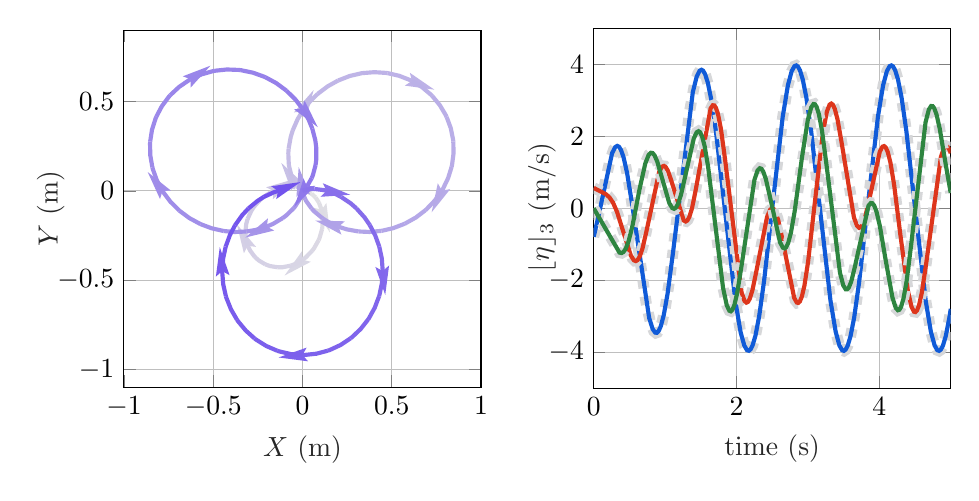
\begin{tikzpicture}

\begin{axis}[%
width=0.374\textwidth,
height=0.374\textwidth,
at={(0\textwidth,0.003\textwidth)},
scale only axis,
xmin=-1,
xmax=1,
xlabel style={font=\color{white!15!black}},
xlabel={$X$ (m)},
ymin=-1.1,
ymax=0.9,
ylabel style={font=\color{white!15!black}},
ylabel={$Y$ (m)},
axis background/.style={fill=white},
xmajorgrids,
ymajorgrids,
ylabel style={yshift=-9.5pt}
]
\addplot [color=mycolor1, line width=1.5pt, forget plot]
  table[row sep=crcr]{%
5.00000499999848e-07	-5.00000499999848e-07\\
0.0265013754917662	-0.00411334835898851\\
};
\addplot [color=mycolor2, line width=1.5pt, forget plot]
  table[row sep=crcr]{%
0.0265013754917662	-0.00411334835898851\\
0.0511086879451376	-0.0164327215387233\\
};
\addplot [color=mycolor3, line width=1.5pt, forget plot]
  table[row sep=crcr]{%
0.0511086879451376	-0.0164327215387233\\
0.0732790863537135	-0.0370569010147855\\
};
\addplot [color=mycolor4, line width=1.5pt, forget plot]
  table[row sep=crcr]{%
0.0732790863537135	-0.0370569010147855\\
0.0925079629951347	-0.0667856880718263\\
};
\addplot [color=mycolor5, line width=1.5pt, forget plot]
  table[row sep=crcr]{%
0.0925079629951347	-0.0667856880718263\\
0.107126731685696	-0.106489066402901\\
};

\addplot[area legend, draw=none, fill=mycolor5, forget plot]
table[row sep=crcr] {%
x	y\\
0.133989136905907	-0.0679278982957864\\
0.107126731685696	-0.106489066402901\\
0.0617002471137037	-0.0944480116554743\\
0.15353693006515	-0.232994623539257\\
}--cycle;
\addplot [color=mycolor6, line width=1.5pt, forget plot]
  table[row sep=crcr]{%
0.107126731685696	-0.106489066402901\\
0.114078837398935	-0.1540036928469\\
0.114168564613308	-0.156167226383796\\
};
\addplot [color=mycolor7, line width=1.5pt, forget plot]
  table[row sep=crcr]{%
0.114168564613308	-0.156167226383796\\
0.110903113067923	-0.207985387622879\\
0.109850589053741	-0.21404469273191\\
};
\addplot [color=mycolor8, line width=1.5pt, forget plot]
  table[row sep=crcr]{%
0.109850589053741	-0.21404469273191\\
0.0952755308686364	-0.264840419838768\\
0.0905779552594511	-0.276050970100925\\
};
\addplot [color=mycolor9, line width=1.5pt, forget plot]
  table[row sep=crcr]{%
0.0905779552594511	-0.276050970100925\\
0.0645151246658051	-0.322153721551351\\
0.0541929993022572	-0.335937453750973\\
};
\addplot [color=mycolor10, line width=1.5pt, forget plot]
  table[row sep=crcr]{%
0.0541929993022572	-0.335937453750973\\
0.0174998178940609	-0.373487090972341\\
0.00109262098511409	-0.386095352497911\\
};

\addplot[area legend, draw=none, fill=mycolor10, forget plot]
table[row sep=crcr] {%
x	y\\
0.0467068212517364	-0.397404518428097\\
0.00109262098511407	-0.386095352497911\\
-0.00389423125228019	-0.339365449814914\\
-0.100475749087956	-0.47464719437994\\
}--cycle;
\addplot [color=mycolor11, line width=1.5pt, forget plot]
  table[row sep=crcr]{%
0.00109262098511409	-0.386095352497911\\
-0.0428719035890877	-0.410720593721746\\
-0.0651504539198176	-0.418928469874351\\
};
\addplot [color=mycolor12, line width=1.5pt, forget plot]
  table[row sep=crcr]{%
-0.0651504539198176	-0.418928469874351\\
-0.111485766763059	-0.427975907194235\\
-0.137905678963928	-0.428460734099644\\
};
\addplot [color=mycolor13, line width=1.5pt, forget plot]
  table[row sep=crcr]{%
-0.137905678963928	-0.428460734099644\\
-0.182479046783407	-0.421228984093121\\
-0.208391057671966	-0.411771559267997\\
};
\addplot [color=mycolor14, line width=1.5pt, forget plot]
  table[row sep=crcr]{%
-0.208391057671966	-0.411771559267997\\
-0.245653115755041	-0.389422016579737\\
-0.267205395068892	-0.369876073357318\\
};
\addplot [color=mycolor15, line width=1.5pt, forget plot]
  table[row sep=crcr]{%
-0.267205395068892	-0.369876073357318\\
-0.293378611815064	-0.334579737168181\\
-0.306152878489832	-0.307793887244029\\
};

\addplot[area legend, draw=none, fill=mycolor15, forget plot]
table[row sep=crcr] {%
x	y\\
-0.328153614965557	-0.349321228773745\\
-0.306152878489832	-0.307793887244029\\
-0.25960344644673	-0.314251663677491\\
-0.367524617408278	-0.187831092336082\\
}--cycle;
\addplot [color=mycolor16, line width=1.5pt, forget plot]
  table[row sep=crcr]{%
-0.306152878489832	-0.307793887244029\\
-0.317622344097296	-0.264183043960445\\
-0.319940411592319	-0.233743960136702\\
};
\addplot [color=mycolor17, line width=1.5pt, forget plot]
  table[row sep=crcr]{%
-0.319940411592319	-0.233743960136702\\
-0.315131074324025	-0.186146967030769\\
-0.307347169100397	-0.157612905295534\\
};
\addplot [color=mycolor18, line width=1.5pt, forget plot]
  table[row sep=crcr]{%
-0.307347169100397	-0.157612905295534\\
-0.286751495407378	-0.112309554229031\\
-0.271582137593871	-0.0890171524312306\\
};
\addplot [color=mycolor19, line width=1.5pt, forget plot]
  table[row sep=crcr]{%
-0.271582137593871	-0.0890171524312306\\
-0.236432881701465	-0.0495934907356708\\
-0.219727559033944	-0.0353752533331661\\
};
\addplot [color=mycolor20, line width=1.5pt, forget plot]
  table[row sep=crcr]{%
-0.219727559033944	-0.0353752533331661\\
-0.175414209824943	-0.00705925990008355\\
-0.161368956879323	-0.000405838455279084\\
};

\addplot[area legend, draw=none, fill=mycolor20, forget plot]
table[row sep=crcr] {%
x	y\\
-0.203797751733084	0.0198018300707399\\
-0.161368956879323	-0.000405838455279077\\
-0.165833420343087	-0.047188538954296\\
-0.0441358110855107	0.0660317414772158\\
}--cycle;
\addplot [color=mycolor21, line width=1.5pt, forget plot]
  table[row sep=crcr]{%
-0.161368956879323	-0.000405838455279084\\
-0.112743500074795	0.0153988328211286\\
-0.106688751621069	0.0166263556465638\\
};
\addplot [color=mycolor22, line width=1.5pt, forget plot]
  table[row sep=crcr]{%
-0.106688751621069	0.0166263556465638\\
-0.0644125702356397	0.0207544614335259\\
};
\addplot [color=mycolor23, line width=1.5pt, forget plot]
  table[row sep=crcr]{%
-0.0644125702356397	0.0207544614335259\\
-0.0400242872580176	0.0202715380062326\\
};
\addplot [color=mycolor24, line width=1.5pt, forget plot]
  table[row sep=crcr]{%
-0.0400242872580176	0.0202715380062326\\
-0.0343623158194826	0.0240276771539405\\
-0.0346064284658818	0.0250169799126352\\
};
\addplot [color=mycolor25, line width=1.5pt, forget plot]
  table[row sep=crcr]{%
-0.0346064284658818	0.0250169799126352\\
-0.044533657950843	0.0443242488501209\\
};

\addplot[area legend, draw=none, fill=mycolor25, forget plot]
table[row sep=crcr] {%
x	y\\
-0.061780695987047	0.000608208556222692\\
-0.044533657950843	0.0443242488501209\\
0.00244516474037955	0.0430821866348205\\
-0.118863119588389	0.156719505123117\\
}--cycle;
\addplot [color=mycolor26, line width=1.5pt, forget plot]
  table[row sep=crcr]{%
-0.044533657950843	0.0443242488501209\\
-0.0620781864684234	0.0850268657023624\\
};
\addplot [color=mycolor27, line width=1.5pt, forget plot]
  table[row sep=crcr]{%
-0.0620781864684234	0.0850268657023624\\
-0.075341046703291	0.139388878578593\\
-0.0768120838628938	0.14990134110874\\
};
\addplot [color=mycolor28, line width=1.5pt, forget plot]
  table[row sep=crcr]{%
-0.0768120838628938	0.14990134110874\\
-0.0793656489201054	0.210589645232636\\
-0.077545754402563	0.23683730449926\\
};
\addplot [color=mycolor29, line width=1.5pt, forget plot]
  table[row sep=crcr]{%
-0.077545754402563	0.23683730449926\\
-0.0660105824112869	0.301024162440814\\
-0.0544494124480615	0.338886965981032\\
};
\addplot [color=mycolor30, line width=1.5pt, forget plot]
  table[row sep=crcr]{%
-0.0544494124480615	0.338886965981032\\
-0.0273736190952321	0.400837288218497\\
-0.000978752731810417	0.445185998229977\\
};

\addplot[area legend, draw=none, fill=mycolor30, forget plot]
table[row sep=crcr] {%
x	y\\
-0.0476170215659137	0.439404616028642\\
-0.000978752731810419	0.445185998229977\\
0.0204168527629962	0.403343668401075\\
0.0621279056164311	0.564245278305569\\
}--cycle;
\addplot [color=mycolor31, line width=1.5pt, forget plot]
  table[row sep=crcr]{%
-0.000978752731810473	0.445185998229977\\
0.0413952250039341	0.499760168425823\\
0.0847322383975153	0.542585372054158\\
};
\addplot [color=mycolor32, line width=1.5pt, forget plot]
  table[row sep=crcr]{%
0.0847322383975153	0.542585372054158\\
0.141113609203002	0.585224842705803\\
0.199250253227126	0.617714426190504\\
};
\addplot [color=mycolor33, line width=1.5pt, forget plot]
  table[row sep=crcr]{%
0.199250253227126	0.617714426190504\\
0.264834961624017	0.643221094037868\\
0.331276730466574	0.658687120775604\\
0.334097454681016	0.659127743172268\\
};
\addplot [color=mycolor34, line width=1.5pt, forget plot]
  table[row sep=crcr]{%
0.334097454681016	0.659127743172268\\
0.402501782176767	0.664601055560168\\
0.468313911196931	0.660417227999415\\
0.476838701816151	0.659180693345462\\
};
\addplot [color=mycolor35, line width=1.5pt, forget plot]
  table[row sep=crcr]{%
0.476838701816151	0.659180693345462\\
0.541145192936933	0.644407089142924\\
0.602547392673032	0.620416030731191\\
0.612822368681951	0.615329041902256\\
};

\addplot[area legend, draw=none, fill=mycolor35, forget plot]
table[row sep=crcr] {%
x	y\\
0.601593653412891	0.66096311309261\\
0.612822368681951	0.615329041902256\\
0.573788103662303	0.589158855537312\\
0.738479819403723	0.566669329838728\\
}--cycle;
\addplot [color=mycolor36, line width=1.5pt, forget plot]
  table[row sep=crcr]{%
0.612822368681951	0.615329041902256\\
0.668990118687385	0.581054758845863\\
0.71924725854335	0.538756862998377\\
0.727293471730299	0.530645994242823\\
};
\addplot [color=mycolor37, line width=1.5pt, forget plot]
  table[row sep=crcr]{%
0.727293471730299	0.530645994242823\\
0.769099859547345	0.480107666901553\\
0.802620396020385	0.423773441585056\\
0.807543038531137	0.413478018418729\\
};
\addplot [color=mycolor38, line width=1.5pt, forget plot]
  table[row sep=crcr]{%
0.807543038531137	0.413478018418729\\
0.830357155287534	0.351995766110661\\
0.843485489000776	0.287666625568427\\
0.84475712296541	0.276297675956115\\
};
\addplot [color=mycolor39, line width=1.5pt, forget plot]
  table[row sep=crcr]{%
0.84475712296541	0.276297675956115\\
0.846207932962063	0.210524137263335\\
0.837745779918826	0.145154077590599\\
0.835280714136298	0.13393617264734\\
};
\addplot [color=mycolor40, line width=1.5pt, forget plot]
  table[row sep=crcr]{%
0.835280714136298	0.13393617264734\\
0.815585281452655	0.0709088520344594\\
0.786943992232661	0.0113746492523306\\
0.781106408162195	0.00147186089867524\\
};

\addplot[area legend, draw=none, fill=mycolor40, forget plot]
table[row sep=crcr] {%
x	y\\
0.827433864739061	0.0093661162225502\\
0.781106408162195	0.0014718608986752\\
0.757831938157076	0.0422989541821901\\
0.723473941732825	-0.120331510619799\\
}--cycle;
\addplot [color=mycolor41, line width=1.5pt, forget plot]
  table[row sep=crcr]{%
0.781106408162195	0.00147186089867524\\
0.74118879953339	-0.0545972269590843\\
0.693768352560731	-0.104102265799389\\
0.689519578575625	-0.107899771911171\\
};
\addplot [color=mycolor42, line width=1.5pt, forget plot]
  table[row sep=crcr]{%
0.689519578575625	-0.107899771911171\\
0.635513146047904	-0.149230125529807\\
0.57447989778035	-0.183512065474833\\
0.571961870061361	-0.184690323792725\\
};
\addplot [color=mycolor43, line width=1.5pt, forget plot]
  table[row sep=crcr]{%
0.571961870061361	-0.184690323792725\\
0.507736446597028	-0.209237686752438\\
0.442293460165524	-0.224363089066711\\
};
\addplot [color=mycolor44, line width=1.5pt, forget plot]
  table[row sep=crcr]{%
0.442293460165524	-0.224363089066711\\
0.374842771314584	-0.230409470600157\\
0.314724136184517	-0.227815521766527\\
};
\addplot [color=mycolor45, line width=1.5pt, forget plot]
  table[row sep=crcr]{%
0.314724136184517	-0.227815521766527\\
0.248979250364356	-0.215978498331708\\
0.20173086625087	-0.201034798221103\\
};

\addplot[area legend, draw=none, fill=mycolor45, forget plot]
table[row sep=crcr] {%
x	y\\
0.217874378622792	-0.245170265912039\\
0.20173086625087	-0.201034798221103\\
0.237674801457332	-0.170759626514346\\
0.0715122473049078	-0.166384058260658\\
}--cycle;
\addplot [color=mycolor46, line width=1.5pt, forget plot]
  table[row sep=crcr]{%
0.20173086625087	-0.201034798221103\\
0.143114764022726	-0.173501555418499\\
0.112278622616077	-0.153988049887413\\
};
\addplot [color=mycolor47, line width=1.5pt, forget plot]
  table[row sep=crcr]{%
0.112278622616077	-0.153988049887413\\
0.0661505900866919	-0.115524233533828\\
0.0506123988726587	-0.0989246960545829\\
};
\addplot [color=mycolor48, line width=1.5pt, forget plot]
  table[row sep=crcr]{%
0.0506123988726587	-0.0989246960545829\\
0.0197503545321327	-0.0556684547100662\\
0.0157993881474753	-0.0483564210491\\
};
\addplot [color=mycolor49, line width=1.5pt, forget plot]
  table[row sep=crcr]{%
0.0157993881474753	-0.0483564210491\\
0.00208479878061224	-0.0130276764482361\\
};
\addplot [color=mycolor50, line width=1.5pt, forget plot]
  table[row sep=crcr]{%
0.00208479878061224	-0.0130276764482361\\
2.9752733209619e-07	-0.000189253426112061\\
};

\addplot[area legend, draw=none, fill=mycolor50, forget plot]
table[row sep=crcr] {%
x	y\\
-0.0337893911652441	-0.0328513023217154\\
2.97527332095506e-07	-0.000189253426112061\\
0.0422550691293849	-0.020758326736749\\
-0.0211624097463592	0.132888552089489\\
}--cycle;
\addplot [color=mycolor51, line width=1.5pt, forget plot]
  table[row sep=crcr]{%
2.9752733209619e-07	-0.000189253426112061\\
-0.00195061487787633	-0.0124397222419582\\
};
\addplot [color=mycolor52, line width=1.5pt, forget plot]
  table[row sep=crcr]{%
-0.00195061487787633	-0.0124397222419582\\
-0.0152935968211821	-0.0473117402838227\\
};
\addplot [color=mycolor53, line width=1.5pt, forget plot]
  table[row sep=crcr]{%
-0.0152935968211821	-0.0473117402838227\\
-0.0423921898581975	-0.0889768920706124\\
-0.0495814778928719	-0.0976657593657855\\
};
\addplot [color=mycolor54, line width=1.5pt, forget plot]
  table[row sep=crcr]{%
-0.0495814778928718	-0.0976657593657855\\
-0.0907234887299729	-0.137607160624197\\
-0.110699935947294	-0.15282989503963\\
};
\addplot [color=mycolor55, line width=1.5pt, forget plot]
  table[row sep=crcr]{%
-0.110699935947294	-0.15282989503963\\
-0.164618301576514	-0.184904772222049\\
-0.199744184780217	-0.200310427997575\\
};

\addplot[area legend, draw=none, fill=mycolor55, forget plot]
table[row sep=crcr] {%
x	y\\
-0.158256827024473	-0.222386470361343\\
-0.199744184780217	-0.200310427997575\\
-0.193201965415219	-0.153772788760284\\
-0.319818127582071	-0.261464420181381\\
}--cycle;
\addplot [color=mycolor56, line width=1.5pt, forget plot]
  table[row sep=crcr]{%
-0.199744184780217	-0.200310427997575\\
-0.262787552507463	-0.219413371362603\\
-0.312642634152668	-0.227809926234432\\
};
\addplot [color=mycolor57, line width=1.5pt, forget plot]
  table[row sep=crcr]{%
-0.312642634152668	-0.227809926234432\\
-0.380588702611795	-0.230659089406199\\
-0.440589302390829	-0.22524258237515\\
};
\addplot [color=mycolor58, line width=1.5pt, forget plot]
  table[row sep=crcr]{%
-0.440589302390829	-0.22524258237515\\
-0.50906055224857	-0.209783802350695\\
-0.571223137222575	-0.186436252548091\\
};
\addplot [color=mycolor59, line width=1.5pt, forget plot]
  table[row sep=crcr]{%
-0.571223137222575	-0.186436252548091\\
-0.63313587577612	-0.152876768025937\\
-0.688200011106969	-0.11212878021732\\
-0.690378128024164	-0.110257884000666\\
};
\addplot [color=mycolor60, line width=1.5pt, forget plot]
  table[row sep=crcr]{%
-0.690378128024164	-0.110257884000666\\
-0.739344135858327	-0.0614739011919233\\
-0.781034398357464	-0.00589093726179712\\
-0.784140555098408	-0.000986362862271939\\
};

\addplot[area legend, draw=none, fill=mycolor60, forget plot]
table[row sep=crcr] {%
x	y\\
-0.797964515322561	-0.0459024025777348\\
-0.784140555098408	-0.000986362862271964\\
-0.737205873678296	0.00139862770220585\\
-0.866917358088304	0.105341260015191\\
}--cycle;
\addplot [color=mycolor61, line width=1.5pt, forget plot]
  table[row sep=crcr]{%
-0.784140555098408	-0.000986362862271939\\
-0.815414366004458	0.0580027739780906\\
-0.837932018704708	0.120891065663995\\
-0.840902245896847	0.132128970587643\\
};
\addplot [color=mycolor62, line width=1.5pt, forget plot]
  table[row sep=crcr]{%
-0.840902245896847	0.132128970587643\\
-0.852319976571281	0.197879644339871\\
-0.853854109958988	0.264498252977816\\
-0.853098534668844	0.276062168862203\\
};
\addplot [color=mycolor63, line width=1.5pt, forget plot]
  table[row sep=crcr]{%
-0.853098534668844	0.276062168862203\\
-0.842884055960361	0.341786549882725\\
-0.822831074838894	0.405118870856366\\
-0.81836679848364	0.415780505086232\\
};
\addplot [color=mycolor64, line width=1.5pt, forget plot]
  table[row sep=crcr]{%
-0.81836679848364	0.415780505086232\\
-0.787321477072651	0.474459185355994\\
-0.747660874220302	0.527710494826103\\
-0.739948811819439	0.536326210765391\\
};
\addplot [color=mycolor65, line width=1.5pt, forget plot]
  table[row sep=crcr]{%
-0.739948811819439	0.536326210765391\\
-0.691360847134042	0.581685287929729\\
-0.636392329891135	0.619228579165222\\
-0.626274447812446	0.624898433672868\\
};

\addplot[area legend, draw=none, fill=mycolor65, forget plot]
table[row sep=crcr] {%
x	y\\
-0.670272378495104	0.641413111860589\\
-0.626274447812446	0.624898433672868\\
-0.626731900708186	0.577905421034305\\
-0.515135988866448	0.701094269799974\\
}--cycle;
\addplot [color=mycolor66, line width=1.5pt, forget plot]
  table[row sep=crcr]{%
-0.626274447812446	0.624898433672868\\
-0.565464878903387	0.652280140347932\\
-0.501207027586293	0.670432248091956\\
-0.489788080333473	0.672623432443533\\
};
\addplot [color=mycolor67, line width=1.5pt, forget plot]
  table[row sep=crcr]{%
-0.489788080333473	0.672623432443533\\
-0.423361390115704	0.679619934047483\\
-0.356702053395848	0.677131866787107\\
-0.345193574936765	0.675748109543327\\
};
\addplot [color=mycolor68, line width=1.5pt, forget plot]
  table[row sep=crcr]{%
-0.345193574936765	0.675748109543327\\
-0.277330016607525	0.661728870696574\\
-0.212590876139102	0.638415168910863\\
-0.207381577421378	0.636079290015891\\
};
\addplot [color=mycolor69, line width=1.5pt, forget plot]
  table[row sep=crcr]{%
-0.207381577421378	0.636079290015891\\
-0.147580372654989	0.603717925834417\\
-0.0914495030501972	0.562399528132818\\
-0.0893505597661588	0.560605399090182\\
};
\addplot [color=mycolor70, line width=1.5pt, forget plot]
  table[row sep=crcr]{%
-0.0893505597661588	0.560605399090182\\
-0.0390747650893384	0.510755976009323\\
-0.000433507010335954	0.460360995528663\\
};

\addplot[area legend, draw=none, fill=mycolor70, forget plot]
table[row sep=crcr] {%
x	y\\
0.0120024085758236	0.505680974605599\\
-0.000433507010335992	0.460360995528663\\
-0.0472726262429882	0.456533540824896\\
0.0855745021058953	0.356629684595743\\
}--cycle;
\addplot [color=mycolor71, line width=1.5pt, forget plot]
  table[row sep=crcr]{%
-0.000433507010336009	0.460360995528663\\
0.0336885295073077	0.400597092791462\\
0.0549048276331719	0.348709143167289\\
};
\addplot [color=mycolor72, line width=1.5pt, forget plot]
  table[row sep=crcr]{%
0.0549048276331719	0.348709143167289\\
0.0717381298533755	0.284154742829256\\
0.0775223484316073	0.239304428039562\\
};
\addplot [color=mycolor73, line width=1.5pt, forget plot]
  table[row sep=crcr]{%
0.0775223484316072	0.239304428039562\\
0.0773375938303877	0.176089617399187\\
0.0732420861311281	0.144047197543308\\
};
\addplot [color=mycolor74, line width=1.5pt, forget plot]
  table[row sep=crcr]{%
0.0732420861311281	0.144047197543308\\
0.0583474020954778	0.0877773436527653\\
0.0517427413978515	0.0713400570273847\\
};
\addplot [color=mycolor75, line width=1.5pt, forget plot]
  table[row sep=crcr]{%
0.0517427413978514	0.0713400570273846\\
0.0274500587337318	0.0283709231246937\\
0.024871722705002	0.0249107592011922\\
};

\addplot[area legend, draw=none, fill=mycolor75, forget plot]
table[row sep=crcr] {%
x	y\\
0.0717803188494607	0.0277631455277734\\
0.024871722705002	0.0249107592011922\\
0.00613566573125181	0.0680096300573571\\
-0.0455596252217695	-0.0899673837556735\\
}--cycle;
\addplot [color=mycolor76, line width=1.5pt, forget plot]
  table[row sep=crcr]{%
0.024871722705002	0.0249107592011922\\
0.00464278981149495	0.00337852674177999\\
};
\addplot [color=mycolor77, line width=1.5pt, forget plot]
  table[row sep=crcr]{%
0.00464278981149495	0.00337852674177999\\
1.25299792142278e-06	7.2114337034291e-07\\
0.00122805843651691	0.000626843304930743\\
};
\addplot [color=mycolor78, line width=1.5pt, forget plot]
  table[row sep=crcr]{%
0.00122805843651691	0.000626843304930742\\
0.0212544728177197	0.00692221502454979\\
};
\addplot [color=mycolor79, line width=1.5pt, forget plot]
  table[row sep=crcr]{%
0.0212544728177197	0.00692221502454979\\
0.0643868643987775	0.0106566520714876\\
0.0666678695800637	0.0106041751411284\\
};
\addplot [color=mycolor80, line width=1.5pt, forget plot]
  table[row sep=crcr]{%
0.0666678695800637	0.0106041751411285\\
0.117874708265099	0.00414994140543432\\
0.134340609456187	8.42911656505629e-05\\
};

\addplot[area legend, draw=none, fill=mycolor80, forget plot]
table[row sep=crcr] {%
x	y\\
0.114124265644782	0.0425089531312935\\
0.134340609456187	8.42911656505703e-05\\
0.101398199115192	-0.0334321242292788\\
0.267237494837189	-0.0221863252611332\\
}--cycle;
\addplot [color=mycolor81, line width=1.5pt, forget plot]
  table[row sep=crcr]{%
0.134340609456187	8.42911656505629e-05\\
0.189258378295869	-0.0201766688175062\\
0.216484732812136	-0.0341555219696192\\
};
\addplot [color=mycolor82, line width=1.5pt, forget plot]
  table[row sep=crcr]{%
0.216484732812136	-0.0341555219696192\\
0.269826194616556	-0.0700177433297552\\
0.301809085267037	-0.0978752405815907\\
};
\addplot [color=mycolor83, line width=1.5pt, forget plot]
  table[row sep=crcr]{%
0.301809085267037	-0.0978752405815907\\
0.347618681220839	-0.148908180826905\\
0.37724469208962	-0.191962215856031\\
};
\addplot [color=mycolor84, line width=1.5pt, forget plot]
  table[row sep=crcr]{%
0.37724469208962	-0.191962215856031\\
0.408240246024384	-0.251645859791259\\
0.429975243642979	-0.312065284774686\\
};
\addplot [color=mycolor85, line width=1.5pt, forget plot]
  table[row sep=crcr]{%
0.429975243642979	-0.312065284774686\\
0.444393705300019	-0.379173999826386\\
0.449462224105245	-0.449038731373988\\
};

\addplot[area legend, draw=none, fill=mycolor85, forget plot]
table[row sep=crcr] {%
x	y\\
0.484930815483934	-0.418208040080868\\
0.449462224105245	-0.449038731373988\\
0.408353533223703	-0.426265325084945\\
0.46356247286238	-0.583048975329392\\
}--cycle;
\addplot [color=mycolor86, line width=1.5pt, forget plot]
  table[row sep=crcr]{%
0.449462224105245	-0.449038731373988\\
0.444897123892077	-0.517128386430186\\
0.430766526366139	-0.584591687027398\\
0.429154201737565	-0.590133703431094\\
};
\addplot [color=mycolor87, line width=1.5pt, forget plot]
  table[row sep=crcr]{%
0.429154201737565	-0.590133703431094\\
0.404639249356969	-0.655055289642328\\
0.372424070198187	-0.713487095310002\\
0.367617123753341	-0.720760446971597\\
};
\addplot [color=mycolor88, line width=1.5pt, forget plot]
  table[row sep=crcr]{%
0.367617123753341	-0.720760446971597\\
0.326384854979144	-0.773315979374907\\
0.277988341417939	-0.819313203270134\\
0.268909933992888	-0.826557262619458\\
};
\addplot [color=mycolor89, line width=1.5pt, forget plot]
  table[row sep=crcr]{%
0.268909933992888	-0.826557262619458\\
0.213370342929258	-0.863429048935478\\
0.153031031202607	-0.891520876313368\\
0.142144152055218	-0.89545474648368\\
};
\addplot [color=mycolor90, line width=1.5pt, forget plot]
  table[row sep=crcr]{%
0.142144152055218	-0.89545474648368\\
0.0778805337052385	-0.912361002661764\\
0.0118445110155938	-0.919261846483617\\
0.000289822454792699	-0.919423879442962\\
};

\addplot[area legend, draw=none, fill=mycolor90, forget plot]
table[row sep=crcr] {%
x	y\\
0.0310912249220421	-0.95491790860352\\
0.00028982245479273	-0.919423879442962\\
0.0230971550497482	-0.878334001371799\\
-0.133732015200719	-0.933413501719477\\
}--cycle;
\addplot [color=mycolor91, line width=1.5pt, forget plot]
  table[row sep=crcr]{%
0.000289822454792699	-0.919423879442962\\
-0.0659084703900581	-0.914376418805691\\
-0.130606106749796	-0.899272807733615\\
-0.141595375810369	-0.895643889701407\\
};
\addplot [color=mycolor92, line width=1.5pt, forget plot]
  table[row sep=crcr]{%
-0.141595375810369	-0.895643889701407\\
-0.202670735846322	-0.86923783312035\\
-0.259180478474166	-0.833907002205977\\
-0.268449485815816	-0.826913340531441\\
};
\addplot [color=mycolor93, line width=1.5pt, forget plot]
  table[row sep=crcr]{%
-0.268449485815816	-0.826913340531441\\
-0.318054022114164	-0.782240354323794\\
-0.360658763508076	-0.73079124442751\\
-0.36729026990346	-0.721242278358795\\
};
\addplot [color=mycolor94, line width=1.5pt, forget plot]
  table[row sep=crcr]{%
-0.36729026990346	-0.721242278358795\\
-0.400657525861906	-0.663440460816566\\
-0.426434371655024	-0.598965747099865\\
-0.428987924662328	-0.590687116509539\\
};
\addplot [color=mycolor95, line width=1.5pt, forget plot]
  table[row sep=crcr]{%
-0.428987924662328	-0.590687116509539\\
-0.444001333961149	-0.523363547359637\\
-0.449434411314596	-0.455263430706976\\
-0.449461863001227	-0.449604387721156\\
};

\addplot[area legend, draw=none, fill=mycolor95, forget plot]
table[row sep=crcr] {%
x	y\\
-0.485017595506882	-0.480334542064834\\
-0.449461863001227	-0.449604387721156\\
-0.408417809538788	-0.472494083555144\\
-0.463182665393183	-0.315554762276991\\
}--cycle;
\addplot [color=mycolor96, line width=1.5pt, forget plot]
  table[row sep=crcr]{%
-0.449461863001227	-0.449604387721156\\
-0.444471413175946	-0.379724239503498\\
-0.430124358078784	-0.312587163276271\\
};
\addplot [color=mycolor97, line width=1.5pt, forget plot]
  table[row sep=crcr]{%
-0.430124358078784	-0.312587163276271\\
-0.406327095022158	-0.247306707147321\\
-0.37750815128357	-0.192395477505825\\
};
\addplot [color=mycolor98, line width=1.5pt, forget plot]
  table[row sep=crcr]{%
-0.37750815128357	-0.192395477505825\\
-0.337313406969777	-0.136040188052468\\
-0.30213889652048	-0.0981922921817903\\
};
\addplot [color=mycolor99, line width=1.5pt, forget plot]
  table[row sep=crcr]{%
-0.30213889652048	-0.0981922921817903\\
-0.251290050093659	-0.0561819031151353\\
-0.216827708134912	-0.0343493736634244\\
};
\addplot [color=mycolor100, line width=1.5pt, forget plot]
  table[row sep=crcr]{%
-0.216827708134912	-0.0343493736634245\\
-0.161477461732493	-0.00863414822557065\\
-0.136181763360186	-0.000428051228803156\\
};

\addplot[area legend, draw=none, fill=mycolor100, forget plot]
table[row sep=crcr] {%
x	y\\
-0.175404832697763	0.0254583029320221\\
-0.136181763360186	-0.000428051228803164\\
-0.147079166355483	-0.0461423718292245\\
-0.0108805825280046	0.0491418648701869\\
}--cycle;
\end{axis}

\begin{axis}[%
width=0.374\textwidth,
height=0.377\textwidth,
at={(0.492\textwidth,0.002\textwidth)},
scale only axis,
xmin=0,
xmax=5,
xlabel style={font=\color{white!15!black}},
xlabel={time (s)},
ymin=-5,
ymax=5,
ylabel style={font=\color{white!15!black}},
ylabel={$\lfloor \eta \rfloor_3$ (m/s)},
axis background/.style={fill=white},
xmajorgrids,
ymajorgrids,
ylabel style={yshift=-9.5pt}
]
\addplot [color=mycolor101, dashed, line width=4.0pt, forget plot]
  table[row sep=crcr]{%
0	-0.794327189375287\\
0.0360072014402881	-0.50936166518636\\
0.127025405081016	0.401132113936494\\
0.228045609121825	1.33632758914924\\
0.281056211242248	1.63329612754323\\
0.317063412682536	1.72220557682937\\
0.341068213642728	1.72499960635367\\
0.366073214642928	1.67811438945176\\
0.398079615923185	1.54390104138956\\
0.441088217643529	1.2377538397163\\
0.498099619923985	0.637283193947144\\
0.585117023404681	-0.56727264865441\\
0.737147429485897	-2.66545859348742\\
0.799159831966393	-3.21078159495211\\
0.843168633726745	-3.41847581720325\\
0.872174434886977	-3.46467191173237\\
0.895179035807161	-3.44825258052759\\
0.922184436887378	-3.3688168708856\\
0.957191438287658	-3.17091411994623\\
1.00320064012803	-2.75704558411858\\
1.06521304260852	-1.95987862632252\\
1.15623124624925	-0.447409965432542\\
1.34126825365073	2.66575265786893\\
1.40928185637127	3.41545782151825\\
1.45829165833167	3.73394012403201\\
1.49329865973195	3.8350088545522\\
1.51630326065213	3.84211915527098\\
1.53930786157231	3.80199999968587\\
1.56931386277255	3.67959099128528\\
1.61032206441288	3.38875659503058\\
1.66333266653331	2.8194308081909\\
1.73434686937387	1.77781972550411\\
1.85837167433487	-0.455471263948239\\
1.98539707941588	-2.59370398474878\\
2.05641128225645	-3.43451931416761\\
2.10942188437688	-3.81699532506429\\
2.14742948589718	-3.9458303120389\\
2.17243448689738	-3.96165841067355\\
2.19543908781756	-3.92756446271101\\
2.2254450890178	-3.81375642817866\\
2.26545309061812	-3.54393669073439\\
2.31746349269854	-3.00700336937391\\
2.38647729545909	-2.02352786337768\\
2.49649929985997	-0.0672605947854992\\
2.64752950590118	2.53899638526069\\
2.71954390878176	3.40814881184364\\
2.77255451090218	3.80338081396424\\
2.81156231246249	3.94419144474996\\
2.8375675135027	3.96432147789867\\
2.86157231446289	3.93010672852998\\
2.89157831566313	3.8167905870463\\
2.93158631726345	3.54778073249147\\
2.98359671934387	3.01205224599861\\
3.05261052210442	2.03014774589095\\
3.1626325265053	0.0753914095624024\\
3.31366273254651	-2.53235407861028\\
3.38667733546709	-3.41325769545288\\
3.43968793758752	-3.80628590341459\\
3.47869573914783	-3.94540123525536\\
3.50370074014803	-3.96476514933784\\
3.52670534106821	-3.93400954089234\\
3.55571114222845	-3.82949823285011\\
3.59471894378876	-3.57687188247151\\
3.64572914582917	-3.06650577686862\\
3.7127425485097	-2.1340631635449\\
3.81576315263053	-0.327947896246553\\
3.98279655931186	2.56766260131723\\
4.05481096219244	3.42712782449802\\
4.10782156431286	3.81387815760879\\
4.14582916583317	3.94626173292067\\
4.17083416683337	3.96459902535318\\
4.19483896779356	3.9304704433463\\
4.2248449689938	3.81727052928625\\
4.26485297059412	3.54842238172358\\
4.31686337267454	3.01289844171149\\
4.38587717543509	2.03121988893501\\
4.49589917983597	0.0766264194557449\\
4.64692938587718	-2.53139747261929\\
4.71994398879776	-3.41262208436514\\
4.77295459091818	-3.80593378247769\\
4.8119623924785	-3.94527327751688\\
4.8369673934787	-3.96478382188333\\
4.85997199439888	-3.93416302561442\\
4.88897779555911	-3.82981902147755\\
4.92798559711942	-3.57740775131461\\
4.97899579915983	-3.06729457175122\\
5	-2.81054586347755\\
};
\addplot [color=mycolor102, line width=1.5pt, forget plot]
  table[row sep=crcr]{%
0	-0.794115885787102\\
0.0600120024004802	-0.281548671295182\\
0.258051610322064	1.53003941505255\\
0.301060212042408	1.69668047404224\\
0.33006601320264	1.73017669989416\\
0.354070814162832	1.70677274522439\\
0.382076415283056	1.62002281949194\\
0.419083816763353	1.40905267100309\\
0.468093618723745	0.973889301725844\\
0.537107421484297	0.121563599122891\\
0.777155431086217	-3.05217301584279\\
0.827165433086617	-3.36333134340827\\
0.862172434486897	-3.45733865837883\\
0.885177035407081	-3.46044900235361\\
0.909181836367273	-3.41338138012364\\
0.940188037607522	-3.27713807917389\\
0.98119623924785	-2.97111617107397\\
1.03520704140828	-2.36976283780686\\
1.10922184436887	-1.25677637678564\\
1.38827765553111	3.2255047963088\\
1.44328865773155	3.66192823178161\\
1.48329665933187	3.81975111046194\\
1.50930186037207	3.84652850865149\\
1.53230646129226	3.81987480647801\\
1.56031206241248	3.72415920730498\\
1.59831966393279	3.48640218969839\\
1.64732946589318	3.00920342715818\\
1.7123424684937	2.1239512497107\\
1.81136227245449	0.41121492337569\\
1.98639727945589	-2.61229059578653\\
2.05741148229646	-3.44625589121601\\
2.10942188437688	-3.81765645670956\\
2.14742948589718	-3.94510072779706\\
2.17243448689738	-3.9599985395867\\
2.19543908781756	-3.92505110274552\\
2.2254450890178	-3.81015031126067\\
2.26545309061812	-3.53894459524268\\
2.31746349269854	-3.00040466253878\\
2.38647729545909	-2.01528674261304\\
2.49749949989998	-0.0392229142670946\\
2.64652930586117	2.53215807614504\\
2.71954390878176	3.41365296862308\\
2.77255451090218	3.8070900644849\\
2.81156231246249	3.94648522689412\\
2.83656731346269	3.9660170022099\\
2.85957191438288	3.93540705306209\\
2.88857771554311	3.83106660798486\\
2.92758551710342	3.57864613467261\\
2.97859571914383	3.06850528074836\\
3.04560912182437	2.13627832251153\\
3.14862972594519	0.330309112130373\\
3.31566313262653	-2.56551901142541\\
3.3876775355071	-3.42521478652696\\
3.44068813762753	-3.81216655078399\\
3.47869573914783	-3.94470336025885\\
3.50370074014803	-3.9631428038853\\
3.52770554110822	-3.9291117650478\\
3.55771154230846	-3.81603117085169\\
3.59671934386877	-3.55563323376992\\
3.64772954590918	-3.03614632651161\\
3.71574314862973	-2.07842654712172\\
3.82276455291058	-0.188077257184159\\
3.98079615923185	2.54658547005319\\
4.05281056211242	3.41367556491065\\
4.10582116423285	3.80718493161305\\
4.14482896579316	3.94667998379694\\
4.16983396679336	3.96629203966992\\
4.19283856771354	3.93576444489673\\
4.22184436887378	3.83153597010651\\
4.26085217043409	3.57927305327881\\
4.3118623724745	3.06933415898445\\
4.37887577515503	2.13733224206793\\
4.48189637927586	0.331540100134837\\
4.64892978595719	-2.56457135084807\\
4.72094418883777	-3.42458628533872\\
4.77395479095819	-3.81182239635184\\
4.8119623924785	-3.94457783568196\\
4.8369673934787	-3.96316392682035\\
4.86097219443889	-3.92927351727076\\
4.89097819563913	-3.81636568318466\\
4.92998599719944	-3.55618191675234\\
4.98099619923985	-3.03694609122357\\
5	-2.79689662272647\\
};
\addplot [color=mycolor101, dashed, line width=4.0pt, forget plot]
  table[row sep=crcr]{%
0	0.563738598755055\\
0.144028805761153	0.422824886409463\\
0.203040608121625	0.338900516746584\\
0.252050410082016	0.219198030896191\\
0.303060612122424	0.0218749578364932\\
0.366073214642928	-0.331414415606499\\
0.543108621724345	-1.39901135571176\\
0.577115423084617	-1.46485997378949\\
0.601120224044809	-1.46165761670337\\
0.627125425085017	-1.40864478511114\\
0.661132226445289	-1.26151278136758\\
0.707141428285658	-0.934761705890972\\
0.780156031206241	-0.212530666000011\\
0.890178035607121	0.843455087591089\\
0.938187637527506	1.10237148930728\\
0.97119423884777	1.17364640492269\\
0.995199039807962	1.16843650901725\\
1.02120424084817	1.11075152641107\\
1.05721144228846	0.951620459176903\\
1.11422284456891	0.565682471698162\\
1.23024604920984	-0.23323299819219\\
1.26925385077015	-0.35305987673321\\
1.29325865173035	-0.365093665906058\\
1.31626325265053	-0.328286677211442\\
1.34526905381076	-0.212929335441658\\
1.38527705541108	0.0671669831279686\\
1.44128825765153	0.65356756811417\\
1.62332466493299	2.70095481449437\\
1.66033206641328	2.85046099163198\\
1.68233646729346	2.86543053501819\\
1.70334066813363	2.82537102894538\\
1.73134626925385	2.68851967879418\\
1.76835367073415	2.3662332609632\\
1.82036407281456	1.67489285280341\\
1.90438087617524	0.185747973705051\\
2.02040408081616	-1.78848733404531\\
2.07641528305661	-2.37765169682113\\
2.11542308461692	-2.58269279836631\\
2.14142828565713	-2.6212654904647\\
2.16343268653731	-2.59435353039503\\
2.19143828765753	-2.48658697753109\\
2.23144628925785	-2.20940010819084\\
2.29445889177836	-1.5726905499727\\
2.41848369673935	-0.308326755793901\\
2.46449289857972	-0.0610044589386494\\
2.49449889977996	-0.00209470576753912\\
2.51650330066013	-0.0135793812990208\\
2.54250850170034	-0.0863409802167192\\
2.57751550310062	-0.279174564286373\\
2.62752550510102	-0.710583759600142\\
2.82156431286257	-2.55708724332431\\
2.85257051410282	-2.63369581823255\\
2.87357471494299	-2.62576767442559\\
2.89757951590318	-2.55454026031909\\
2.92958591718344	-2.35556942661592\\
2.97259451890378	-1.91000377509792\\
3.03160632126425	-1.02299139058083\\
3.25265053010602	2.57473534884735\\
3.29465893178636	2.84319348094709\\
3.32266453290658	2.90327207123327\\
3.34366873374675	2.88585088048239\\
3.36867373474695	2.79805788752941\\
3.40368073614723	2.56326474638185\\
3.45469093818764	2.03288074127015\\
3.66773354670934	-0.405265348152578\\
3.70374074814963	-0.532551629030824\\
3.72674534906981	-0.546649385905505\\
3.74974994999	-0.509138252706884\\
3.77975595119024	-0.387479313389922\\
3.82276455291058	-0.0906015163895262\\
3.89577915583117	0.614912030438296\\
3.98979795959192	1.46770820367028\\
4.03380676135227	1.6821490650085\\
4.06181236247249	1.72483486707426\\
4.08381676335267	1.70140370211403\\
4.10982196439288	1.60678307853976\\
4.14482896579316	1.36615688347012\\
4.19283856771354	0.843703045075206\\
4.26485297059412	-0.239009788805682\\
4.40288057611522	-2.32572239080855\\
4.45289057811562	-2.75146671330331\\
4.4868973794759	-2.87773440588151\\
4.50690138027606	-2.88546251286034\\
4.52890578115623	-2.83653094921302\\
4.55791158231646	-2.68255338108008\\
4.59791958391678	-2.31683476454457\\
4.65593118623725	-1.53652495221267\\
4.85797159431886	1.39002978701013\\
4.90198039607922	1.65874659199883\\
4.93198639727946	1.72342149461871\\
4.95399079815963	1.71042408658685\\
4.97999599919984	1.63301945331375\\
5	1.53476369707534\\
};
\addplot [color=mycolor103, line width=1.5pt, forget plot]
  table[row sep=crcr]{%
0	0.564186778452506\\
0.170034006801361	0.390416241509775\\
0.222044408881777	0.298114320082673\\
0.271054210842168	0.15338131243091\\
0.326065213042608	-0.0962195972077406\\
0.400080016003201	-0.562471769858115\\
0.520104020804161	-1.31490510814333\\
0.563112622524505	-1.44830800233186\\
0.590118023604721	-1.46896428676708\\
0.614122824564913	-1.44165034099659\\
0.643128625725145	-1.34957578994217\\
0.682136427285458	-1.12769521874752\\
0.737147429485897	-0.656800087245514\\
0.918183636727345	1.01627313806796\\
0.957191438287658	1.15415247348467\\
0.983196639327866	1.175977119315\\
1.00720144028806	1.14671489143587\\
1.03820764152831	1.04383957972942\\
1.08221644328866	0.794486194193295\\
1.26125225045009	-0.340813599116563\\
1.28825765153031	-0.368986988909137\\
1.31126225245049	-0.342209455500238\\
1.33926785357071	-0.244349763487643\\
1.37727545509102	-1.15216419729336e-05\\
1.42928585717143	0.512845780439928\\
1.6373274654931	2.77270937792024\\
1.66833366673335	2.85931589898962\\
1.68833766753351	2.8556144382997\\
1.71034206841368	2.79554482474733\\
1.74034806961392	2.61913348931805\\
1.78135627125425	2.21085354382144\\
1.83836767353471	1.37604339150682\\
2.07041408281656	-2.33545498510551\\
2.11142228445689	-2.57332027597161\\
2.13842768553711	-2.62336716384408\\
2.16043208641728	-2.60300173807406\\
2.18643728745749	-2.5125767733585\\
2.22344468893779	-2.27498429039729\\
2.28045609121824	-1.72647355627781\\
2.42748549709942	-0.245100872647233\\
2.47049409881976	-0.0419591221697928\\
2.49849969993999	-0.000682620909299381\\
2.52050410082016	-0.0209572416537673\\
2.54750950190038	-0.108173592776233\\
2.58451690338068	-0.330798159017057\\
2.63852770554111	-0.825398811139285\\
2.80756151230246	-2.48964827027343\\
2.84356871374275	-2.62005052676997\\
2.86557311462292	-2.63202191531771\\
2.88657731546309	-2.59212796347232\\
2.91458291658332	-2.4591929741845\\
2.95159031806361	-2.14638236285467\\
3.00260052010402	-1.4858360530042\\
3.08161632326465	-0.106095050971176\\
3.21064212842569	2.11443050220311\\
3.26565313062613	2.68567095534497\\
3.30366073214643	2.8773182021258\\
3.32766553310662	2.90752583446832\\
3.34866973394679	2.87696826872694\\
3.37567513502701	2.7632681897713\\
3.41368273654731	2.47612684274774\\
3.47069413882777	1.83360978934093\\
3.64472894578916	-0.257860532951248\\
3.6877375475095	-0.489785804088418\\
3.71674334866973	-0.544408155380985\\
3.73874774954991	-0.530383108513651\\
3.76475295059012	-0.454629498502783\\
3.80076015203041	-0.254409953838413\\
3.85477095419084	0.203923266554534\\
4.00680136027205	1.57291685810258\\
4.04480896179236	1.71020048066954\\
4.06781356271254	1.72477123428655\\
4.08981796359272	1.68661240259526\\
4.11782356471294	1.56281375454684\\
4.15583116623325	1.26357288985989\\
4.20784156831366	0.63924886766925\\
4.29485897179436	-0.742712398223539\\
4.39787957591518	-2.27175373969661\\
4.4498899779956	-2.73505216460452\\
4.48489697939588	-2.87465986873214\\
4.50590118023605	-2.88611385790756\\
4.52690538107622	-2.8427153658298\\
4.55591118223645	-2.69483364305717\\
4.59491898379676	-2.34747289709997\\
4.65193038607722	-1.59419296701138\\
4.8629725945189	1.43155172607768\\
4.90498099619924	1.66916868879035\\
4.93398679735947	1.72304906623893\\
4.95599119823965	1.70488850868468\\
4.98199639927986	1.6218438310574\\
5	1.52876874271121\\
};
\addplot [color=mycolor101, dashed, line width=4.0pt, forget plot]
  table[row sep=crcr]{%
0	-0.0017710012859995\\
0.147029405881177	-0.492822672620548\\
0.363072614522904	-1.2359777377815\\
0.392078415683137	-1.2467292359574\\
0.419083816763353	-1.21470389339174\\
0.451090218043609	-1.11869030325354\\
0.492098419683937	-0.900883749609628\\
0.546109221844369	-0.467302625005596\\
0.661132226445289	0.716665260247203\\
0.731146229245849	1.29320871444687\\
0.775155031006201	1.49194431348794\\
0.805161032206441	1.53880937419337\\
0.829165833166633	1.52353277168502\\
0.857171434286857	1.44957813831848\\
0.896179235847169	1.25957765195701\\
0.96119223844769	0.79898309397691\\
1.05721144228846	0.148071322324303\\
1.09921984396879	0.00493263493341001\\
1.12622524504901	-0.0177222479103403\\
1.1502300460092	0.0114239256117123\\
1.18023604720944	0.112827830487295\\
1.22124424884977	0.358067586554899\\
1.28425685137027	0.907517771066531\\
1.40128025605121	1.93223769348852\\
1.44228845769154	2.10947883467689\\
1.46829365873175	2.13969239371206\\
1.49029805961192	2.10970047150483\\
1.51730346069214	2.0003829051319\\
1.55331066213243	1.73095247705797\\
1.60232046409282	1.15688973975967\\
1.67633526705341	-0.0318383960839741\\
1.8123624724945	-2.21696674677695\\
1.86437287457492	-2.69810143310115\\
1.8993798759752	-2.84613959938399\\
1.92138427685537	-2.8618955924353\\
1.94238847769554	-2.82143218379132\\
1.97039407881576	-2.68639401482927\\
2.00940188037608	-2.358511229461\\
2.06741348269654	-1.63906316130706\\
2.250450090018	0.784549375690095\\
2.29445889177836	1.04617253025771\\
2.3244648929786	1.11164881877328\\
2.34646929385877	1.10127210863207\\
2.37147429485897	1.03238948793327\\
2.40648129625925	0.844468352410404\\
2.45949189837968	0.405073660542816\\
2.61452290458092	-0.968754222483723\\
2.65253050610122	-1.10036262353954\\
2.6755351070214	-1.11309294553306\\
2.69853970794159	-1.07195231943393\\
2.72754550910182	-0.942487067798342\\
2.76655331066213	-0.637920309070049\\
2.82156431286257	0.00539414545732697\\
3.03560712142429	2.74524302889465\\
3.07061412282456	2.88420028914881\\
3.09161832366473	2.89686418990952\\
3.1126225245049	2.8549034359484\\
3.14062812562512	2.71465036916205\\
3.17863572714543	2.37846619179036\\
3.23264652930586	1.65673752447774\\
3.33066613322665	-0.04638232813807\\
3.4246849369874	-1.51851930551882\\
3.47869573914783	-2.04430919850604\\
3.51670334066813	-2.2264289608395\\
3.54170834166833	-2.25824241570243\\
3.5627125425085	-2.23267986775032\\
3.59071814362873	-2.12954629589037\\
3.63072614522905	-1.86451578971923\\
3.69473894778956	-1.24833437836325\\
3.81076215243049	-0.135590543804457\\
3.85577115423085	0.0928181287552476\\
3.88477695539108	0.144650389269956\\
3.90678135627125	0.130144504310928\\
3.93278655731146	0.0528044584935596\\
3.96779355871174	-0.149374790812371\\
4.01680336067213	-0.593256453675824\\
4.11182236447289	-1.73016766256653\\
4.18983796759352	-2.53461236614931\\
4.23384676935387	-2.785329737115\\
4.2618523704741	-2.83927619232056\\
4.28285657131426	-2.82026405285618\\
4.30786157231446	-2.72892966359937\\
4.34186837367473	-2.48562278681227\\
4.3878775755151	-1.95361121698318\\
4.45289057811562	-0.892463515140784\\
4.6369273854771	2.26759672606397\\
4.68593718743749	2.69468847827867\\
4.71994398879776	2.82582483620396\\
4.74094818963793	2.83789276550784\\
4.7629525905181	2.79591500821677\\
4.79295859171834	2.65481141994948\\
4.83496699339868	2.3182557260575\\
4.90398079615923	1.53662884756745\\
5	0.427830998659389\\
};
\addplot [color=mycolor104, line width=1.5pt, forget plot]
  table[row sep=crcr]{%
0	-0.00177205505912159\\
0.361072214442888	-1.23306810963685\\
0.391078215643129	-1.24585608843917\\
0.418083616723345	-1.21480767033216\\
0.449089817963593	-1.12400964765873\\
0.489097819563913	-0.916841452142505\\
0.542108421684337	-0.49970122462711\\
0.641128225645129	0.518759975595833\\
0.722144428885777	1.23937638113678\\
0.769153830766153	1.47727465537583\\
0.801160232046409	1.53966392839888\\
0.825165033006601	1.53157644372441\\
0.852170434086817	1.46870980392987\\
0.890178035607121	1.2955142476367\\
0.949189837967594	0.891480591164352\\
1.05921184236847	0.139208400298235\\
1.1002200440088	0.0042113743694161\\
1.12622524504901	-0.0162079109352256\\
1.1502300460092	0.013293346213846\\
1.18023604720944	0.115114402318137\\
1.22124424884977	0.360801218982242\\
1.28425685137027	0.910461516074635\\
1.40128025605121	1.93354402050587\\
1.44228845769154	2.10965376585778\\
1.46829365873175	2.13905816548654\\
1.49029805961192	2.10835097434197\\
1.51730346069214	1.99814612427206\\
1.55331066213243	1.72757403494472\\
1.60232046409282	1.15216721129046\\
1.67633526705341	-0.0377911645686053\\
1.81136227245449	-2.20998873959137\\
1.86337267453491	-2.69546189483418\\
1.8993798759752	-2.84889288850012\\
1.92038407681536	-2.86462643403034\\
1.94138827765553	-2.826117985964\\
1.96939387877576	-2.69353978069039\\
2.00840168033607	-2.36862104180861\\
2.06641328265653	-1.65212989379109\\
2.25145029005801	0.792021200549065\\
2.29545909181836	1.04819219702099\\
2.3254650930186	1.10980915481232\\
2.34746949389878	1.09668338142833\\
2.37347469493899	1.02081992232456\\
2.40948189637928	0.819697254442284\\
2.46449289857972	0.352085164317502\\
2.60952190438088	-0.946011794481395\\
2.64852970594119	-1.09591064533065\\
2.67353470694139	-1.11658937012207\\
2.69553910782156	-1.08234177263378\\
2.72354470894179	-0.966640820597833\\
2.76155231046209	-0.685117574931967\\
2.81456291258252	-0.0870031564348022\\
2.91358271654331	1.36625236211351\\
2.99759951990398	2.44205908739713\\
3.04560912182437	2.79839598188369\\
3.07761552310462	2.89247325610494\\
3.09861972394479	2.88638192067064\\
3.12162432486497	2.81698525187545\\
3.15263052610522	2.62187403949004\\
3.19563912782557	2.17377446948158\\
3.25765153030606	1.24466197250153\\
3.44868973794759	-1.79224810996018\\
3.49569913982797	-2.14779874862191\\
3.52870574114823	-2.25127640245108\\
3.55071014202841	-2.25321998550123\\
3.57371474294859	-2.20070652476498\\
3.60672134426885	-2.0371703440337\\
3.65373074614923	-1.66053441414842\\
3.84876975395079	0.0709487671976401\\
3.88077615523105	0.144071219663896\\
3.90278055611122	0.137714772556467\\
3.92778555711142	0.0736766344046345\\
3.96079215843169	-0.0999568133812039\\
4.00680136027205	-0.489974052316338\\
4.08381676335267	-1.38538843728836\\
4.18383676735347	-2.48531535430221\\
4.22984596919384	-2.76796144786039\\
4.25985197039408	-2.83485592334778\\
4.28085617123425	-2.82012435295655\\
4.30486097219444	-2.73885785130325\\
4.3378675735147	-2.51515900874972\\
4.38187637527505	-2.02775979373526\\
4.44388877775555	-1.04663309065522\\
4.64692938587718	2.38303144050851\\
4.69293858771754	2.7381041546463\\
4.7249449889978	2.83747147818966\\
4.74594918983797	2.83653161119381\\
4.76895379075815	2.77781151024405\\
4.80096019203841	2.60394609688219\\
4.84696939387878	2.19871136732769\\
4.93198639727946	1.18897651419594\\
5	0.423006539024289\\
};
\end{axis}
\end{tikzpicture}%
  \includegraphics*{./pdf/thesis-figure-4-5.pdf}
  \caption{(left) The forward kinematics of the end-effector $\vec{\gamma}$ related to the prescribed reference $\q_d(t)$. The time evolution is shown by the colormap \protect\colormapcaption{0}{.75cm}$\!\!\in [0,5]$ (s). (right) The linear velocities $\floor{\etaB}_3 = (v_1,\,v_2,\,v_3)^\top$, shown as (\ldata{Matlab1},\ldata{Matlab2},\ldata{Matlab3}), respectively. The dashed lines (\ldata{lightgrey}) are obtained using numerical time differentiation of $\vec{\gamma}$ -- and the overlap exactly with the forward kinematic model. A key observation here, is that our numerical approach prevents the common numerical instability for near-zero curvatures, \ie, $\kappa \to 0$, since the linear velocities are bounded and continuous even for $\kappa(\q) = 0$. }
  \label{fig:C2:EX1:strain_ref_FK}
\end{figure}
\vfill

\begin{figure}[!h]
   \centering
   %\vspace{-2mm}
   %% This file was created by matlab2tikz.
%
%The latest updates can be retrieved from
%  http://www.mathworks.com/matlabcentral/fileexchange/22022-matlab2tikz-matlab2tikz
%where you can also make suggestions and rate matlab2tikz.
%
\begin{tikzpicture}

\begin{axis}[%
width=0.216\textwidth,
height=0.199\textwidth,
at={(0\textwidth,0.253\textwidth)},
scale only axis,
axis on top,
xmin=0.5,
xmax=522.5,
tick align=outside,
y dir=reverse,
ymin=0.5,
ymax=458.5,
axis line style={draw=none},
ticks=none,
ylabel style={yshift=-7.5pt}
]
\addplot [forget plot] graphics [xmin=0.5, xmax=522.5, ymin=0.5, ymax=458.5] {./fig/fig_plotrobot-1.png};
\end{axis}

\begin{axis}[%
width=0.216\textwidth,
height=0.199\textwidth,
at={(0.245\textwidth,0.253\textwidth)},
scale only axis,
axis on top,
xmin=0.5,
xmax=522.5,
tick align=outside,
y dir=reverse,
ymin=0.5,
ymax=458.5,
axis line style={draw=none},
ticks=none,
ylabel style={yshift=-7.5pt}
]
\addplot [forget plot] graphics [xmin=0.5, xmax=522.5, ymin=0.5, ymax=458.5] {./fig/fig_plotrobot-2.png};
\end{axis}

\begin{axis}[%
width=0.216\textwidth,
height=0.199\textwidth,
at={(0.49\textwidth,0.253\textwidth)},
scale only axis,
axis on top,
xmin=0.5,
xmax=522.5,
tick align=outside,
y dir=reverse,
ymin=0.5,
ymax=458.5,
axis line style={draw=none},
ticks=none,
ylabel style={yshift=-7.5pt}
]
\addplot [forget plot] graphics [xmin=0.5, xmax=522.5, ymin=0.5, ymax=458.5] {./fig/fig_plotrobot-3.png};
\end{axis}

\begin{axis}[%
width=0.216\textwidth,
height=0.199\textwidth,
at={(0.734\textwidth,0.253\textwidth)},
scale only axis,
axis on top,
xmin=0.5,
xmax=522.5,
tick align=outside,
y dir=reverse,
ymin=0.5,
ymax=458.5,
axis line style={draw=none},
ticks=none,
ylabel style={yshift=-7.5pt}
]
\addplot [forget plot] graphics [xmin=0.5, xmax=522.5, ymin=0.5, ymax=458.5] {./fig/fig_plotrobot-4.png};
\end{axis}

\begin{axis}[%
width=0.216\textwidth,
height=0.199\textwidth,
at={(0\textwidth,0\textwidth)},
scale only axis,
axis on top,
xmin=0.5,
xmax=522.5,
tick align=outside,
y dir=reverse,
ymin=0.5,
ymax=458.5,
axis line style={draw=none},
ticks=none,
ylabel style={yshift=-7.5pt}
]
\addplot [forget plot] graphics [xmin=0.5, xmax=522.5, ymin=0.5, ymax=458.5] {./fig/fig_plotrobot-5.png};
\end{axis}

\begin{axis}[%
width=0.216\textwidth,
height=0.199\textwidth,
at={(0.245\textwidth,0\textwidth)},
scale only axis,
axis on top,
xmin=0.5,
xmax=522.5,
tick align=outside,
y dir=reverse,
ymin=0.5,
ymax=458.5,
axis line style={draw=none},
ticks=none,
ylabel style={yshift=-7.5pt}
]
\addplot [forget plot] graphics [xmin=0.5, xmax=522.5, ymin=0.5, ymax=458.5] {./fig/fig_plotrobot-6.png};
\end{axis}

\begin{axis}[%
width=0.216\textwidth,
height=0.199\textwidth,
at={(0.49\textwidth,0\textwidth)},
scale only axis,
axis on top,
xmin=0.5,
xmax=522.5,
tick align=outside,
y dir=reverse,
ymin=0.5,
ymax=458.5,
axis line style={draw=none},
ticks=none,
ylabel style={yshift=-7.5pt}
]
\addplot [forget plot] graphics [xmin=0.5, xmax=522.5, ymin=0.5, ymax=458.5] {./fig/fig_plotrobot-7.png};
\end{axis}

\begin{axis}[%
width=0.216\textwidth,
height=0.199\textwidth,
at={(0.734\textwidth,0\textwidth)},
scale only axis,
axis on top,
xmin=0.5,
xmax=522.5,
tick align=outside,
y dir=reverse,
ymin=0.5,
ymax=458.5,
axis line style={draw=none},
ticks=none,
ylabel style={yshift=-7.5pt}
]
\addplot [forget plot] graphics [xmin=0.5, xmax=522.5, ymin=0.5, ymax=458.5] {./fig/fig_plotrobot-8.png};
\end{axis}
\end{tikzpicture}%
   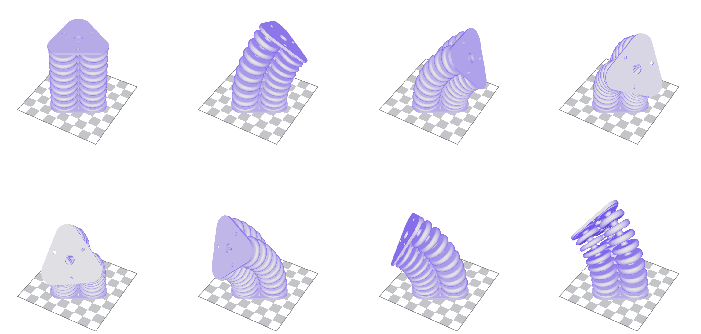
\includegraphics[width=.95\textwidth]{./pdf/thesis-figure-4-4.pdf}
   %\vspace{-2mm}
   \caption{Three-dimensional deformation of the three-bellow soft robot manipulator using the PCC model. Based on the prescribed reference $\q_d$ (and its time-derivative $\dq_d$), the forward kinematic relations for each point $\sigma$ along the backbone is computed and the volumetric mesh is deformed accordingly to its closest material-point on $\gammaB(\sigma)$.}
   \vspace{-0.1cm}
   \label{fig:C2:EX1:strain_ref_3D}
 \end{figure}

\subsection{Piecewise curve dynamics using Euler-Lagrange}
\noindent Given the forward kinematics in \eqref{eq:C2:phi_exact}, \eqref{eq:C2:pos_exact}, \eqref{eq:C2:vel_cont} and \eqref{eq:C2:acceleration}, we can shift our attention to formulating the finite-dimensional dynamics of the soft robot. Our goal here is to write the spatio-temporal dynamics of the hyper-elastic soft robot as a second-order ODE into the Lagrangian form:
%
% \begin{equation}
% \frac{d}{d t}\left(\frac{\partial \mathcal{L}}{\partial \dq} \right) - \frac{\partial \mathcal{L}}{\partial \q} = \vec{Q}^{\nc}, \label{eq:euler_largrange}
% \end{equation}
%
\begin{equation}
\frac{d}{d t}\left(\grad{\dq} \Lf \right) - \grad{\q} \Lf = \vec{Q}^{\nc}, \label{eq:C2:euler_largrange}
\end{equation}
%
\noindent where the mathematical operator $\grad{\vec{x}} (\cdot) := \p(\cdot)^\top/\p \vec{x}$ denotes the gradient w.r.t. to $\xB$, $\La(\q,\dq) := \Kf(\q,\dq) - \mathcal{U}(\q)$ the Lagrangian function, $\Kf \in \Rp$ and $\mathcal{U}\in \R$ the kinetic and potential energy, respectively; and $\vec{Q}^{\nc} \in \R^n$ a vector of generalized non-conservative forces. To apply the Lagrangian formalism to a continuum dynamical system,  consider an infinitesimal slice of the continuum body for each material coordinate $\sigma$ along the backbone curve. Given this notion, we assign the infinitesimal slice with an inertia tensor $\ten{M} = \text{blkdiag}(\rho_0 \mat{I},\ten{J}_{\!0})$ with $\rho_0 = m_0/L$ the line-density and $\ten{J}_{\!0} \in \coso{3} \times \sog{3}$ a symmetric tensor related to the second moment of inertia of infinitesimal slice at $\sigma$.  Note that operator $\text{blkdiag}(\cdot)$ creates a block diagonal matrix by aligning the input matrices.

The kinetic energy can be obtained through spatial integration of its respective kinetic energy densities \cite{Boyer2010,Mochiyama2003,Tatlicioglu2007}, \ie,
$\mathfrak{T} = \frac{1}{2}\etaB^\top \ten{M} \etaB
$:
%
\begin{align}
\mathcal{T}({\q},\dot{{\q}}) & = \frac{1}{2}\int_\Xs \etaB(\sigma,{\q},\dot{\q})^\top\,\ten{M}\,{\etaB}(\sigma,{\q},\dot{{\q}}) \; d \sigma,
 \notag \\[0.35em]
& =  \frac{1}{2} \dot{\q}^\top \left[\int_\Xs  \JB(\sigma,\q)^\top\,\ten{M}\, \JB(\sigma,\q) \; d \sigma \right]\, \dot{\q} := \frac{1}{2}\dot{\q}^\top \mat{M}(\q) \dot{\q},
\label{eq:C2:kinetic_energy}
\end{align}
%
% \begin{rmk}[Generalized inertia for zero-curvature]
% Given the form of the generalized inertia matrix  \eqref{eq:C2:kinetic_energy}, and assuming $\JB(\cdot,\q)$ to be full-rank for all $\q \in \Q$ we can easily show that $\lambda^{-} \preceq \mat{M}(\q) \preceq \lambda^{+} < \infty$ with $\lambda^{-}$ and $\lambda^{+}$
% positive constants.
% \end{rmk}
%
where we used $\etaB = \JB \q$ as described in \eqref{eq:C2:vel_cont}. Also note that expression for the kinetic energy naturally gives rise to the generalized inertia matrix $\MB(\q)$ of the Lagrangian model. By substitution of the kinetic energy into the Euler-Lagrange equation \eqref{eq:C2:euler_largrange}, we find $\MB(\q)\ddq + \CB(\q,\dq)\q$ where $\CB(\q,\dot{\q})$ denotes the Coriolis matrix.  Instead of computing the Coriolis matrix through the conventional Christoffel symbols \cite{Murray1994}, we a modified computational scheme introduced by Garofalo et al. \cite{Garofalo2013} that is tailored towards long serial-chain manipulators. In their scheme, we replaced the finite summation of $N$ rigid bodies by a spatial integration over the continuum domain $\Xs$. This leads to the following computation of the Coriolis matrix: 
%
\begin{multline}
\mat{C}(\q,\dq) = \int_\Xs \JB(\sigma,\q)^\top \overbrace{\left[\ten{M} \ad_{\etaB}  - \ad_{\etaB} ^\top \ten{M} \right]}^{\ten{C}_{\etaB}} \JB(\sigma,\q)\; +\; ... \\[0.35em] ...\; + \JB(\sigma,\q)^\top \ten{M} \,\,\dot{\!\!\JB}(\sigma,\q,\dq) \; d \sigma,
\label{eq:C2:coriolis}
\end{multline}
%
where $\ten{C}_{\etaB} = -\ten{C}_{\etaB}^\top$ a skew-symmetric matrix. The computation above is slight different from existing literature \cite{Boyer2021,Renda2020} to ensure that the matrix $\dot{\mat{M}} - 2\mat{C}$ is skew-symmetric -- the so-called "\emph{passivity condition}"(see Assumption \ref{as:C2:passivity}). The importance of this property will become apparent later in the energy-based controller design. Lastly, the potential energy is given by sum of gravitational potential energy and internal elastic potential, \ie,
$\mathcal{U}(\q) = \mathcal{U}\grav(\q) + \mathcal{U}\elastic(\q)
$. Since gravitational potential energy density is given by $\mathfrak{U}_g = -\rho_0\,\gammaB(\sigma,\q) \vec{a}_g$ with $\vec{a}_g \in \R^3$ is a vector of body accelerations, the potential energy related to gravity is obtained by spatial integration of their respective energy densities:
%
\begin{equation}
\mathcal{U}\grav(\q) = \int_\Xs \mathfrak{U}\grav(\sigma,\q) \; d\sigma = - \rho_0 \int_\Xs \,\gammaB(\sigma,\q)^\top \vec{a}_g \; d \sigma.
\label{eq:C2:potential_energy_grav}
\end{equation}
%
\noindent To model the hyper-elastic nature, lets introduce two nonlinear stiffness functions for both stretching and bending, denoted by $k_e: \R \mapsto \Rsp$ and $k_b: \R \mapsto \Rsp$, respectively. These functions allow us to describe a collective elastic behavior imposed by the hyper-elastic materials and the continuum-bodied deformation. It shall be clear that these entities are unique to the soft robot's geometry and soft material choice, and thus finding a suitable candidate model requires further analysis. Later, we will sculpt these nonlinear stiffness functions through Finite Element Methods (FEM). For now, we assume that these analytical nonlinear stiffness functions are known, and thus the (hyper)-elastic potential energy takes the form
%
\begin{equation}
\mathcal{U}_e(\q) = \int_0^{\varepsilon} k_e(s) \,s \; d s + \int_0^{\beta(\q)} k_b(s)\, s \; d s,
\label{eq:C2:potential_energy_elas}
\end{equation}
%
where $\varepsilon$ is the elongation strain, and $\beta(\q) := \kappa L(\varepsilon + 1)$ is the bending angle with the total curvature of the segment $\kappa(\q) = || \kappa_x, \,\kappa_y ||_2$ (see Figure \ref{fig:C2:configuration}).

\subsection{Overall dynamic model}
\noindent Finally, by combining \eqref{eq:C2:euler_largrange}, \eqref{eq:C2:kinetic_energy}, \eqref{eq:C2:coriolis}, \eqref{eq:C2:potential_energy_grav}, and \eqref{eq:C2:potential_energy_elas}, the continuum dynamics of the soft robot can be casted into the familiar closed form
\cite{DellaSantina2020,Boyer2021,Renda2018} similar to aforementioned model (1):
%
\begin{align}
\mat{M}(\q)\,\ddq + \mat{C}(\q,\dq)\,\dq + \fB\!\elastic(\q,\dq) + \fB\!\grav(\q) & = \tauB(\uB,\vec{\delta}),
\label{eq:C2:dynamic_model}
\end{align}
%
where $\fB\elastic = \grad{\q}\Uf_{\textrm{e}} + \mat{R}\dq$ is a vector of generalized forces imposed by the deformation of the soft materials with $\vec{R} \succ 0$ the Rayleigh damping matrix,
$\vec{f}\grav = \grad{\q} \mathcal{U}\grav$ a vector of generalized gravitational forces, and
$\uB(t)$ the control input with the index
$m$ the number of pressure inputs. The generalized input vector is chosen of the form:
$\tauB(\uB,\vec{\delta}) = \mat{G}\uB + \vec{\delta}$ with $\mat{G} \uB: \R^m \to \R^n$ a mapping from the input space to the joint actuation space, and $\vec{\delta}(t)$ an external disturbance (\eg, unmodelled material uncertainties).
%
\begin{rmk}
Given the context of  pick-and-place applications in robot manipulators , a possible disturbance $\vec{\delta}(t)$ could be an external mass applied to the tip of the soft robot.  Given the kinematic relations in \eqref{eq:C2:vel_cont} and \eqref{eq:C2:acceleration}, one can describe the disturbance (modeled here as a point-mass located at $L$) as an external wrench acting on the point $\sigma = L$. The disturbance has two part related to acceleration: \textit{(i)} the gravitational acceleration expressed in the body-frame ${\normalfont \Ad}_{\gB(\cdot,L)}\inv \aB_g$ and \textit{(ii)} the acceleration due to the tip motion $\dot{\etaB}(\cdot,L)$. Together they form a state-dependent vector as follows: 
%
\begin{equation}
\vec{\delta}_m = m_\delta \floor{\JB(\cdot,L)}_3^\top\left({\normalfont \Ad}_{\gB(\cdot,L)}\inv \aB_g + \floor{\dot{\etaB}(\cdot,L)}_3 \right),
\label{eq:C2:delta_payload}
\end{equation}
%
where $m_\delta > 0$ the applied mass to the end-effector, $\floor{\cdot}_3$ extracts the last three rows of a matrix or vector. Recall that the acceleration twist can be computed through the geometric Jacobian and its time derivative, i.e., $\dot{\etaB} = \JB\ddq + \JB\dq$. Indeed, the PCC condition for a soft body can only accurately describe the true dynamics if external forces produced by mass $m_\delta$ do not excessively exceed the intrinsic elastic balancing forces $\vec{f}\!\elastic(\q)$. Alternatively, a soft body can be modeled using multiple PCC curves of smaller size, similar to standard Finite Element discretization.
\end{rmk}

\begin{asm}[Input mapping of bellows]  Uptil now, we have not specific the input map $\GB$. In general, the input map is difficult to properly estimate as the system's inputs are distributed over the soft continuum body. Therefore, it involves integrating the actuation wrench along the backbonce curve, while accounting for the spatial dependency of the geometric manipulator Jacobian $\JB(\q,\sigma)$. However, we considering the soft robotic system in Figure \ref{fig:C2:soft_robot}, we can introduce some approximations for the actuation mapping $\mat{G}$ based on the geometry, placement, and orientation of the (pneumatic) soft actuators. Since the pneumatic chambers are aligned parallel to the backbone curve and are equally spaced along the circumference, we propose the following ansatz: 
%
\begin{equation}
\vec{G} \simeq \begin{pmatrix} \alpha_{\varepsilon} & \hdots & \alpha_{\varepsilon} \\ -\alpha_{\kappa} \cos(\phi_1) & \hdots & -\alpha_{\kappa} \cos(\phi_m) \\ \alpha_{\kappa} \sin(\phi_1) & \hdots & \alpha_{\kappa} \sin(\phi_m) \end{pmatrix},
\label{eq:C2:mapping_H}
\end{equation}
%
where $\alpha_{\varepsilon},\alpha_{\kappa} > 0$ are system parameters representing the effective transferal of differential pressure to joint forces, and $\phi_i = (i-1)\cdot\tfrac{2\pi}{m}$ the angular inter-distance between the $m$-number of pneumatic bellows. Please note that the parameters $\alpha_{\varepsilon}$ and $\alpha_{\kappa}$ are dependent on the bellow area and radius from the bellow to the backbone curve.
\end{asm}